\documentclass[12pt]{article}
\usepackage{animate}
\usepackage{url}
\usepackage[export]{adjustbox}
\usepackage{subcaption}
%\usepackage{fixltx2e}
\usepackage{caption}
\usepackage{listings}
\usepackage{color}
\usepackage{animate}
\usepackage{media9}
\definecolor{dkgreen}{rgb}{0,0.6,0}
\definecolor{gray}{rgb}{0.5,0.5,0.5}
\definecolor{mauve}{rgb}{0.58,0,0.82}

\lstset{frame=tb,
	language=R,
	aboveskip=3mm,
	belowskip=3mm,
	showstringspaces=false,
	columns=flexible,
	basicstyle={\small\ttfamily},
	numbers=left,
	numberstyle=\tiny\color{black},
	keywordstyle=\color{blue},
	commentstyle=\color{gray},
	stringstyle=\color{dkgreen},
	breaklines=true,
	breakatwhitespace=true,
	tabsize=3
}


\def\ContinueLineNumber{\lstset{firstnumber=last}}
\def\StartLineAtOne{\lstset{firstnumber=1}}
\let\numberLineAt\StartLineAt



\usepackage[english]{babel}
\usepackage{natbib}
\usepackage{url}
\usepackage[utf8x]{inputenc}
\usepackage{amsmath}
\usepackage[absolute,overlay]{textpos}
\usepackage{verbatim}
\usepackage{fancyvrb}
\usepackage{float}
\usepackage{graphicx}
\graphicspath{{images/}}
\usepackage{parskip}
\usepackage{fancyhdr}
\usepackage{vmargin}
\usepackage{authblk}
\usepackage{ragged2e}

\setmarginsrb{3 cm}{2.5 cm}{3 cm}{2.5 cm}{1 cm}{1.5 cm}{1 cm}{1.5 cm}

\title{ Life Insurance using R Technical Documentation }		%					% Author
\date{\today}											% Date
\makeatletter
\let\thetitle\@title
\let\theauthor\@author
\let\thedate\@date
\makeatother

\pagestyle{fancy}
\fancyhf{}
%\rhead{\theauthor}
\lhead{\thetitle}
\cfoot{\thepage}




\begin{document}
	
	%%%%%%%%%%%%%%%%%%%%%%%%%%%%%%%%%%%%%%%%%%%%%%%%%%%%%%%%%%%%%%%%%%%%%%%%%%%%%%%%%%%%%%%%%
	
	\begin{titlepage}
		\centering
		\vspace*{0.1 cm}
		
\includegraphics[scale = 0.2]{cwu.PNG}\\[1.0 cm]
		%\includegraphics[scale = 0.75]{logo2.jpg}\\[1.0 cm]	% University Logo
		\textsc{\LARGE Central Washington University}\\[2.0 cm]	% University Name
		\textsc{\Large CS 567}\\[0.5 cm]	% Course Code
		\textsc{\large Computational Statistics}\\[0.5 cm]	% Course Name
		\rule{\linewidth}{0.2 mm} \\[0.4 cm]
		{ \huge \bfseries \thetitle}\\
		\rule{\linewidth}{0.2 mm} \\[1.5 cm]
		
		\begin{minipage}{0.4\textwidth}
			\begin{flushleft} \large
				%\emph{Authors:}\\
				Chao Huang  \\
				41716747\\
				Hermann Yepdjio\\
				40917845\\
				Lubna Alzamil\\
				41442408
			\end{flushleft}
		\end{minipage}~
		\begin{minipage}{0.4\textwidth}
			\begin{center} \large
\emph{Instructor:} \\
Dr.Donald \textsc{Davendra}					
			\end{center}
		\end{minipage}\\[1 cm]
		
		{\large \thedate}\\[1 cm]
		
		\vfill
		
	\end{titlepage}
	
	%%%%%%%%%%%%%%%%%%%%%%%%%%%%%%%%%%%%%%%%%%%%%%%%%%%%%%%%%%%%%%%%%%%%%%%%%%%%%%%%%%%%%%%%%
	
	\tableofcontents
	\pagebreak
	\lstlistoflistings
	\listoffigures
	%\listoftables
	\pagebreak
	
	
	%%%%%%%%%%%%%%%%%%%%%%%%%%%%%%%%%%%%%%%%%%%%%%%%%%%%%%%%%%%%%%%%%%%%%%%%%%%%%%%%%%%%%%%%%
	
	\section{Introduction}
This project implements the formulas used by life insurance companies using the R programming language version 3.5.1. Applying the equations into the computer will make it easier and more efficient to calculate and visualize several types of products offered by the insurance companies. 
\section{Overview}
The data used is a mortality data taken from the Society of Actuaries Mortality Tables. The mortality data was downloaded and saved as a CSV file called compare.csv.  All the equations were coded in an R file called life-table.R.  The user can specify the inputs by editing life-table-inputs.txt. The life-table .R reads the data from the life-table-inputs.txt file and outputs the result. The project also simulates the production of life insurance policies for 10000 clients.  The process takes place in project1-updated.R file. Additionally, the code calculates the profit and the fund value that the company earns depending on the interests and the benefits paid. Furthermore, the code generates plots of a variety of variables that will help the company to visualize the results of the calculations.
\section{The Code}
\subsection{Life-table.R}
\begin{lstlisting}[caption={ Reading The Data Part 1},captionpos=b]
startTime <- Sys.time()
setwd("/media/hermann/Tonpi/tonpi/Collegecourses/CWU/Graduate School/Winter 2019/CS 567/Projects/Project1/3R")
inputs <- read.table("life_table_inputs.txt", header = TRUE, sep = "\t", dec = ".", stringsAsFactors=FALSE) #read the inputs values from the life_table_inputs.txt file
inputMortalityFile <- (inputs[inputs$label == "inputMortalityFile", c("value")])
print (inputMortalityFile)
data <- read.csv(inputMortalityFile, header = TRUE, stringsAsFactors=FALSE) #avoid convert string to factor
dataTotalRow <- nrow(data)
beginRowData = 1
\end{lstlisting}
In Listing 1, Line 1 stores the start time when the code is started to execute. At the end of code execution, the total time will be printed. Line 2 sets the working directory. Line 3 reads the inputs values from the life-table-inputs.txt file and store them in \textit{inputs}. Line 4 gets the value of inputMortalityFile row from \textit{inputs} data frame which is compare.csv and stores it in \textit{inputMortalityFile}.Line 5 prints the value of \textit{inputMortalityFile}. Line 6 reads the csv data of inputMortalityFile and store them in \textit{data}. stringsAsFactors=FALSE means that do not covert the string data to factors. Line 7 counts the number of rows in \textit{data}.
\begin{lstlisting}[caption={ Reading The Data Part 2},captionpos=b]
ages = as.numeric(data[beginRowData:dataTotalRow, 1])
mortality = as.numeric(data[beginRowData:dataTotalRow, 2])

lifeTable <- data.frame(ages,mortality)

lifeTableTotalRow = nrow(lifeTable)
lifeTable$t <- lifeTable$ages + 1
lifeTable$q <- lifeTable$mortality
lifeTable$p <- 1 - lifeTable$q
\end{lstlisting}
in Listing 2, line 1 starts to loop inside the first column (ages column) of\textit{data} data frame from 1 until the total rows of \textit{data} then convert the ages into numeric values and store them in \textit{ages}. Line 2 does the same with the second column ,which contains the mortality, storing them as numeric values in \textit{mortality}. Line 4 creates a data frame called \textit{lifeTable} which contains for now two columns \textit{ages} and \textit{mortality}. Line 6 counts the number of rows in \textit{lifeTable} and store them in \textit{lifeTableTotalRow}. Line 7 adds new column to the data frame \textit{lifeTable} the column is called \textit{t} and contains the values ages+1. Line 8 adds new column to the data frame \textit{lifeTable} the column is called \textit{q} and contains the same data as \textit{mortality} column. Line 9 as well adds new column to the data frame \textit{lifeTable} the column is called \textit{p} and contains the values of 1-\textit{q}.
\pagebreak
\StartLineAtOne
\begin{lstlisting} [caption={ Imeplemening The Equations Part 1},captionpos=b]
#calculate v^t
interest <- as.numeric(inputs[inputs$label == "interest", c("value")])
lifeTable$vt <- 1/(1+interest)^lifeTable$t

#calculate t_p_x | x=0
lifeTable$t_p_x0[1] <-  lifeTable$p[1]
for (i in 2:lifeTableTotalRow) {
lifeTable$t_p_x0[i] <- lifeTable$t_p_x0[i-1] *  lifeTable$p[i]
}
\end{lstlisting}
In Listing 3, lines 1 gets the value of interest from \textit{inputs} and stores it in \textit{interest}. Line 2 add new column to the data frame \textit{lifeTable} the column is called $v^{t}$ which contains the value of equation 1 . Lines 6-8 add new column to the data frame \textit{lifeTable} the column is called $_{t}P_{x0}$ and contains the value of equation 2.

\begin{equation}
v^t=(1+i)^{-t}
\end{equation}
\begin{equation}
%\textsubscript{t}p\textsubscript{t}
 %_tp_x=p_x*_t_-_1p_x_=_0 
 _{t}p_{x}=lx_{n}/lx_{n-1}
\end{equation}

\StartLineAtOne
\begin{lstlisting}[caption={Imeplemening The Equations Part 2},captionpos=b]
#calculate t_E_x | x=0
lifeTable$t_E_x0 <- lifeTable$vt * lifeTable$t_p_x0

#calculate a_x
lifeTable$a_x[1] <- 1 + sum(lifeTable$t_E_x0)
for (i in 2:lifeTableTotalRow) {
lifeTable$a_x[i] <- 1 + sum(lifeTable$t_E_x0[i:lifeTableTotalRow])/lifeTable$t_E_x0[i-1]
}

#calculate A_x
d = interest/(1 + interest)
lifeTable$A_x <- 1 - d * lifeTable$a_x
\end{lstlisting}
In Listing 4, line 2 adds new column to the data frame \textit{lifeTable} the column is called $_{t}E_{x0}$ and contains the value $_{t}E_{x}=v^t$ *  $_{t}p_{x0}$. Lines 5-7 add new column to the data frame \textit{lifeTable} the column is called $ax$ and its values are $ax=1+\Sigma _{t}E_{x}$.The first value in  $ax$ column is$=1+\Sigma _{t}E_{x0}$. Lines 11-12 add new column to the data frame \textit{lifeTable} the column is called $A_{x}$ and contains the value of $A_{x}=1-d$ * $ax$.

\subsection{Projec1.R}
\hspace{1 cm}In this file, we are calling the formulas located in life-table.R using the source function.
\StartLineAtOne
\begin{lstlisting}[caption={ The Relationship between $A_{x}$ and Ages},captionpos=b]
setwd(C://Desktop//Statis//GroupProject1//3R)
inputsProject1 <- read.delim("project1_inputs.txt", header = TRUE, sep = "\t", dec = ".", stringsAsFactors=FALSE) #read the inputs values from the project1_inputs.txt file
print (inputsProject1)
source("life_table.R")
#install library if not exist
if (!require(ggplot2)) install.packages('ggplot2')
if (!require(reshape)) install.packages('reshape')
library(ggplot2)
library(reshape)
x11()
myGraph <- ggplot(lifeTable, aes(ages, A_x))
myGraph <- myGraph + geom_point()
print(myGraph)
ggsave(filename = "images/A_x Vs Ages.png", plot = myGraph)
\end{lstlisting}
%%%%%%%%%%%%%%%%%%%%%%%%%%%%%%%%%%%%%%%%%%%%%%%%%
%%%%%%%%%%%%%%%%%%%%%%%%%%%%%%%%%%%%%%%%%%%%%%%%%
%%%%%%%%%%%%%%%%%%%%%%%%%%%%%%%%%%%%%%%%%%%%%%%%%
In Listing 5, line 1 sets the working directory to the path of where the project and needed files are stored . Line 2 reads the inputs values from the project1-inputs.txt file and stores them in \textit{inputsProject1}. Line 3 prints the values in \textit{inputsProject1}. Line 4 calls Life-table.R file that contains the necessary formulas. Line 5-6  install the needed packages and call them with library function . Here we are calling ggplot2 and reshape libries in lines 8-9. Reshape library  is used to cast a data frame into the reshaped form. The library ggplot2 is used for creating plots. Line 10 opens a new graph window before creating a new graph to avoid overwriting of previous plotted graphs. X11() function is used in Unix platform, windows() is used in Windows platform and quartz() is used in Mac platform. Line 11 myGraph contains plots the \textit{ages} and $A_{x}$ cloumns from \textit{lifeTable} data frame. Line 12 geom point function is used to create scatter points displaying the relationship between \textit{ages} and $A_{x}$. Line 13 shows the plot on the screen. Line 14 saves the plot on images folder. Figure 1 shows the result of Line 12.
%%%%%%%%%%%%%%%%%%%%%%%%%%%%%%%%%%%%%%%%%%%%%%%%%
%%%%%%%%%%%%%%%%%%%%%%%%%%%%%%%%%%%%%%%%%%%%%%%%%
%%%%%%%%%%%%%%%%%%%%%%%%%%%%%%%%%%%%%%%%%%%%%%%%%
\begin{figure}[h]
	
	\centering
	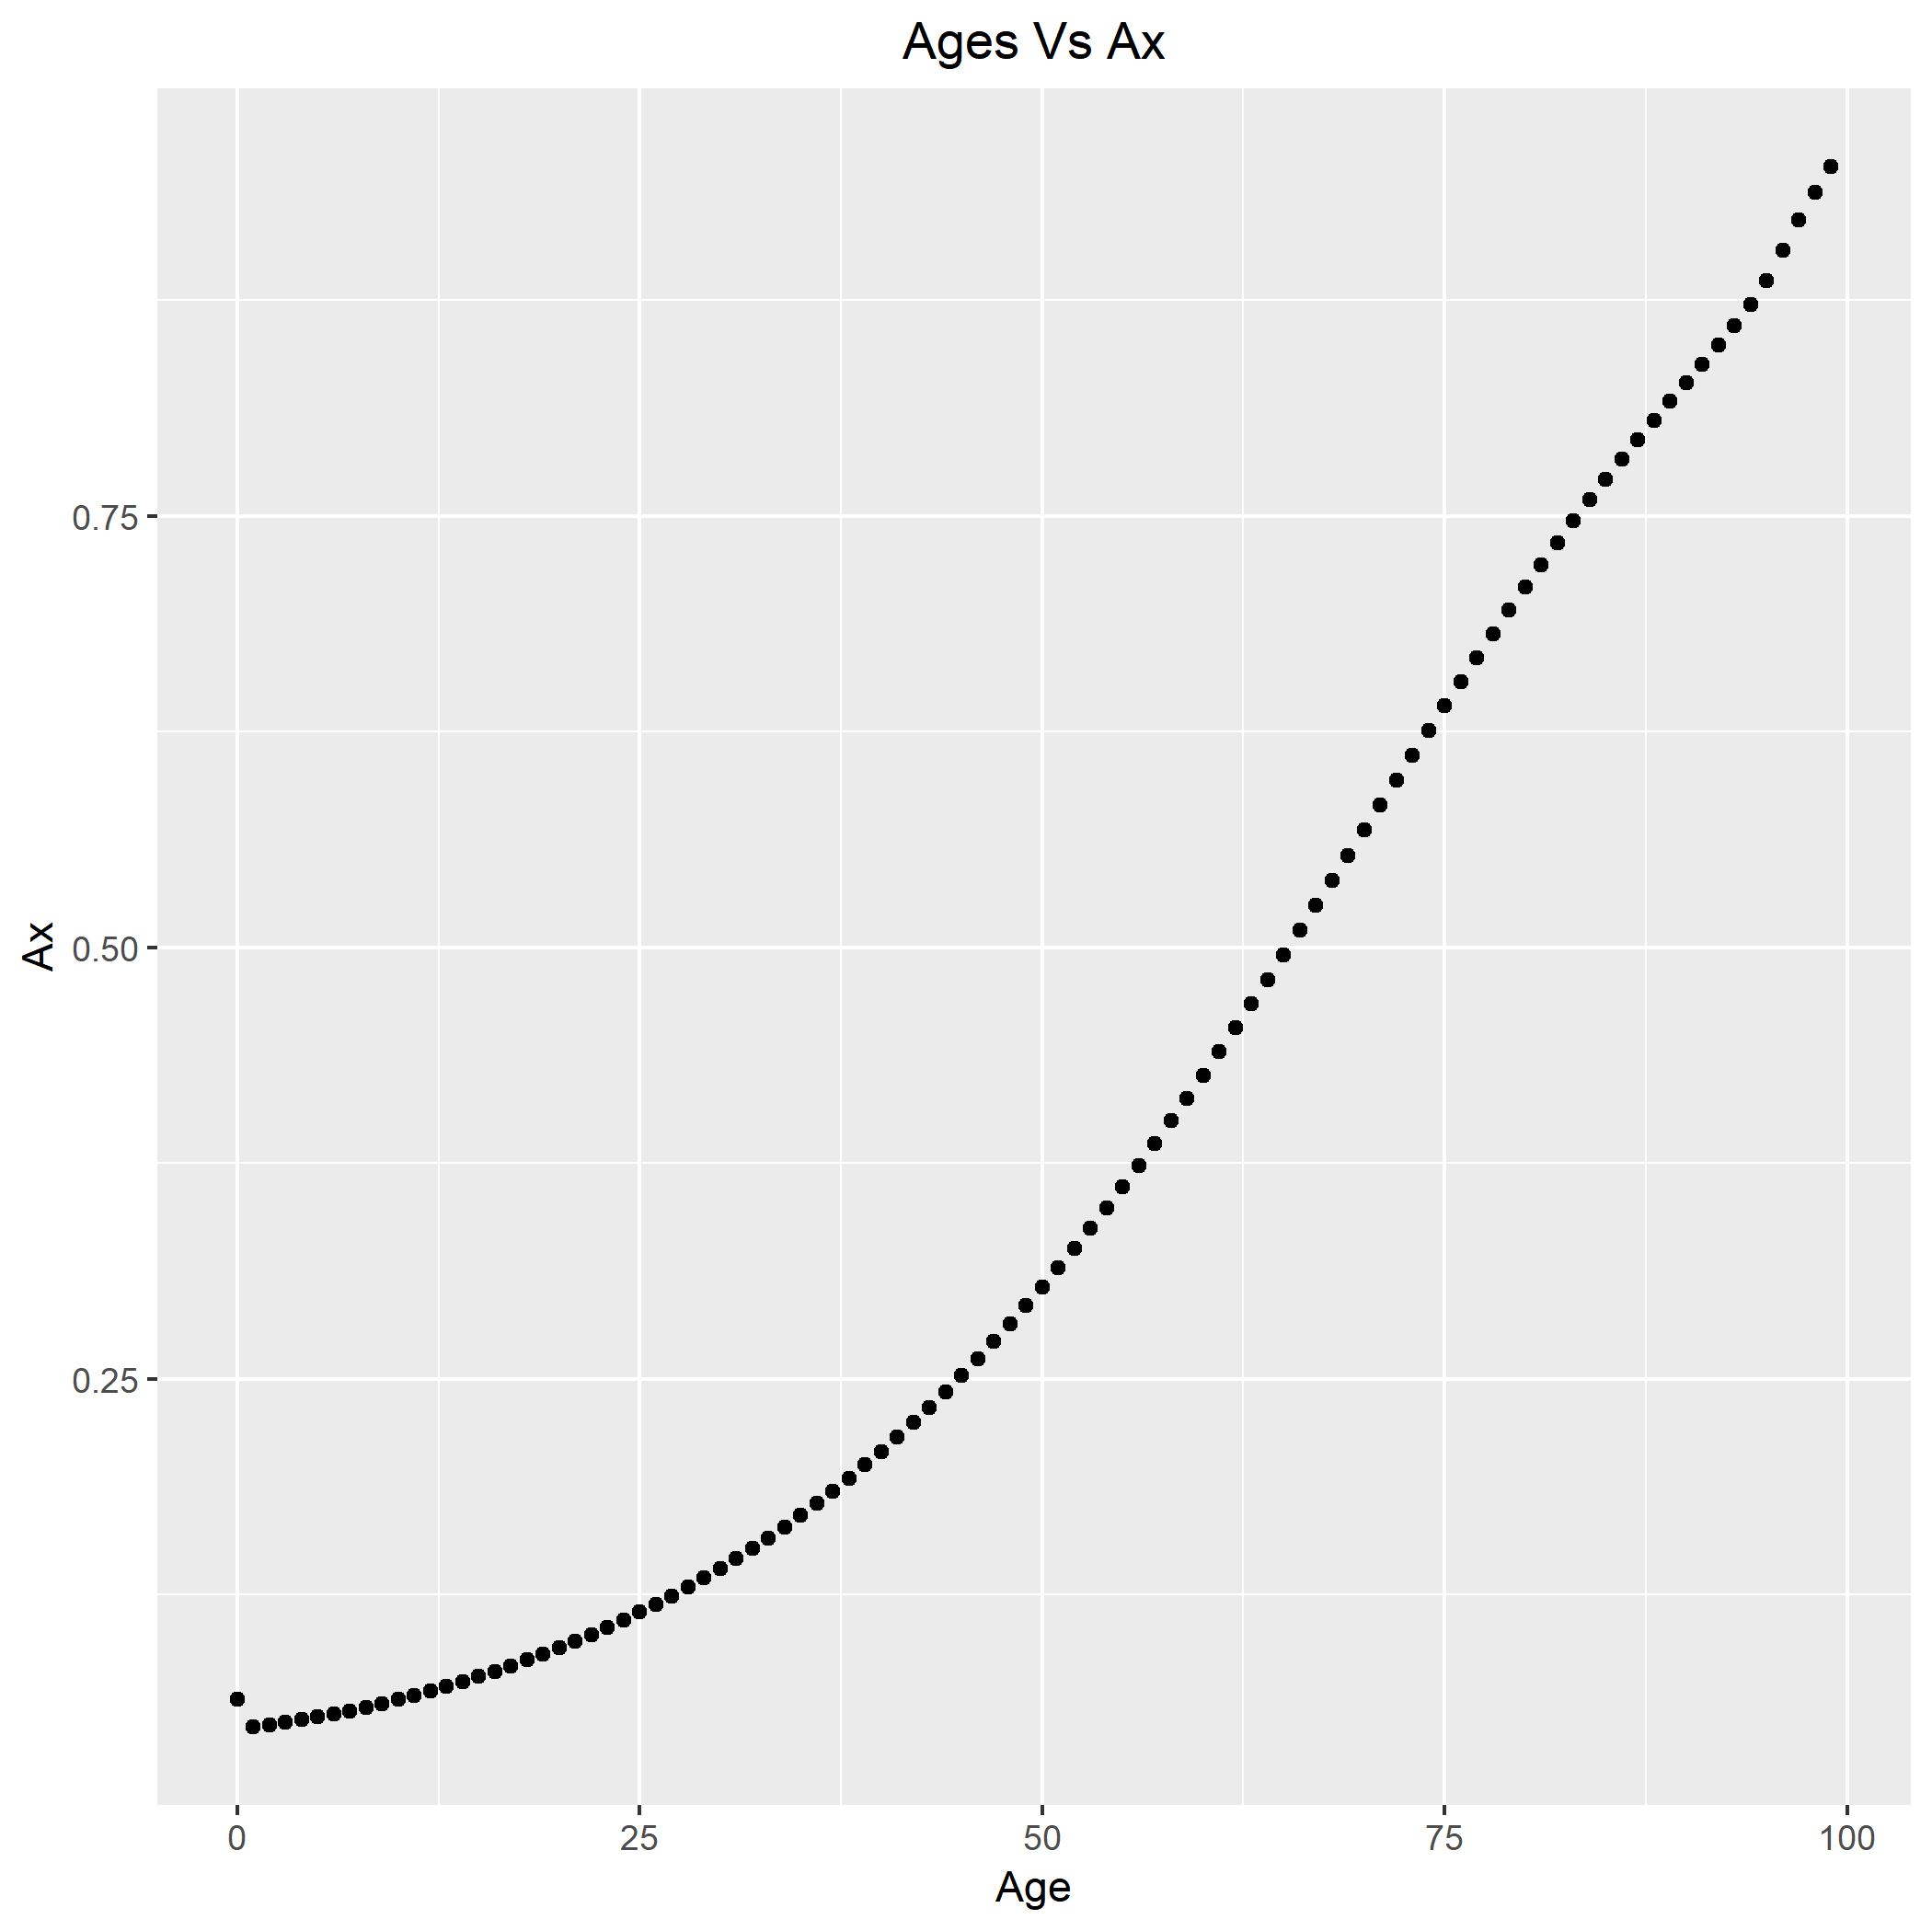
\includegraphics[width=0.5\linewidth, height=5cm]{S1.png}
	
	
	\caption{The Relationship between $A_{x}$ and Ages }
	
\end{figure}

\StartLineAtOne
\begin{lstlisting}[caption={ Life Net Single Premium},captionpos=b]
inputAges = as.numeric(inputsProject1[inputsProject1$label == "inputAges", c("value")])
inputBenefit = as.numeric(inputsProject1[inputsProject1$label == "inputBenefit", c("value")])
nsp <- lifeTable[lifeTable$ages == inputAges, c("A_x")]*inputBenefit
print(paste("input Ages: ", inputAges))
print(paste("Whole Life Net Single Premium: ", nsp))
\end{lstlisting}
In Listing 6, lines 1-2 get the values of inputAges and inputBenefit columns in \textit{inputsProject1} convert them to numeric and store them in \textit{inputAges} and \textit{inputBenefit}. Line 3 extracts the corresponding $A_{x}$ of the \textit{inputAges} which is 12 and multiples it by the \textit{inputBenefit} which is 1000 storing the result in \textit{nsp}. The formula used is $Net Single Premium = Benefit$ * $A_{x}$. Line 4 prints the age. Line 5 prints the result of Net Single Premium.
\pagebreak



%%%%%%%%%%%%%%%%%% S
\pagebreak
\StartLineAtOne
\begin{lstlisting}[caption={ Calculating $_{t}q_{x}$},captionpos=b]
CalculateFinalAgeSemiPerfectData <- function(inputAge) { #---only for testing

#calculate probability of (x) lives t years  t_p_x where x = inputAges
previousAgeP <- lifeTable[ages == (inputAge - 1), c("t_p_x0")]
if (inputAge > 0) {
pLives <- lifeTable[ages >= inputAge, c("t_p_x0")]/previousAgeP
} else {
pLives <- lifeTable[ages >= inputAge, c("t_p_x0")]
}

pLivesAges <- lifeTable[ages >= inputAge, c("ages")]
pCurveX <- data.frame(pLivesAges, pLives)

#calculate probability tl1_q_x that x survives t years and dies within 1 year
pCurveXRow <- nrow(pCurveX)

#probability of dead based on input age
pCurveX$tl1_q_x[1] <- 1 - pCurveX$pLives[1] # firt data important,,, to avoid bug
for (j in 2:(pCurveXRow)) {

#small bug which does not consider the 0|1_q_x data..... also add q_x of 1 in the last year automatically? 
pCurveX$tl1_q_x[j] <- pCurveX$pLives[j-1] - pCurveX$pLives[j]
#pCurveX$tl1_q_x[j] <- pCurveX$pLives[j] - pCurveX$pLives[j+1] #i = u in the pdf   1 = t in pdf
}
#note: return a vector
bFAge <- sample(pCurveX$pLivesAges, inputNumberClients, replace = T, pCurveX$tl1_q_x)


return(bFAge)
}
\end{lstlisting}
Listing 7 calulates the probability of (x) lives t years using the defined function CalculateFinalAgeSemiPerfectData. It finds the probablity $_{t}p_{x0}$ of \textit{inputAges - 1} and stores the result in \textit{previousAgeP}. Then checks whether the \textit{inputAges} is greater than zero or not. If it is, it will get all the probabilities $_{t}p_{x0}$ of all ages and divide by \textit{previousAgeP} and store the result in \textit{pLives}. If the \textit{inputAges} is not greater than zero, it will get all the probabilities $_{t}p_{x0}$ of all ages and store them in \textit{pLives}. Then stores all the ages that are greater than or equal to \textit{inputAges} in \textit{pLivesAges}. After that, it creates a data frame called \textit{pCurveX} that has two columns \textit{pLivesAges} and \textit{pLives}. After that, calculate $_{t1}q_{x}$ which is the probability that x survives t years and dies within 1 year. The general formula used to calculate this probability is\\ $_{u|t}q_{x}=_{u}p_{x}$ - $_{u+t}p_{x}$.  \textit{pCurveXRow} stores the number of rows in \textit{pCurveX} data frame. It iterates from 1 until \textit{pCurveXRow}-1. Adds new column to the data frame \textit{pCurveX} the column is called $_{t1}q_{x}$ and contains the values of the formula $_{u|t}q_{x}=_{u}p_{x}$ - $_{u+t}p_{x}$. Finally, it stores the $_{u|t}q_{x}$ of the last row in \textit{pCurveX} data frame.


%%%%%%%%%%%%%%%%%

%%%%%%%%%%%%%%%%%%%
\StartLineAtOne
\begin{lstlisting}[caption={ 10000 Simulation},captionpos=b]
#now creating a block of 10000 people who are in different ages and want different benefits
BussinessBlock <- function(rAge,rBenefit) { 
netSinglePremium <- lifeTable[lifeTable$ages == rAge, c("A_x")]*rBenefit
return(netSinglePremium)
}

inputNumberClients <- as.numeric(inputsProject1[inputsProject1$label == "inputNumberClients", c("value")])

bAge <- vector(mode="integer", length=inputNumberClients) #initialize variables
bBen <- vector(mode="integer", length=inputNumberClients)
bNps <- vector(mode="numeric", length=inputNumberClients)
bFAge <- vector(mode="integer", length=inputNumberClients)
maxAges <- max(lifeTable$ages)
lifeTableAges <- lifeTable$ages[ages < maxAges]# avoid picking max ages

#looping 10000
lifeTableAges <- data.frame(Age=ages) # creating a data frame that contains the ages
print("---------Calculating Lifetimes-----------")
print(paste("Number of clients: ", inputNumberClients))
lifeTableAsVector = as.vector(lifeTable[1,], mode = 'numeric') #create a vector representation of lifeTable so I can pass it to the c function
for (i in 2:lifeTableTotalRow)
{
lifeTableAsVector = c(lifeTableAsVector, as.vector(lifeTable[i,], 
mode = 'numeric'))
}
dim = c(length(lifeTableAges$Age), 10, length(lifeTableAges$Age)) #bug if only put lifeTableAges -> length =1, 99 instead of 100
dyn.load("c_code.dll")
res = .C("for_loop", lifeTable=as.numeric(lifeTableAsVector), dim = as.integer(dim), bAge = as.numeric(bAge), bBen=as.integer(bBen), bNps = as.numeric(bNps), bFAge = as.numeric(bFAge), lifeTableAges = as.integer(lifeTableAges), inputNumberClients =as.integer(inputNumberClients))
bFAge = res[6]$bFAge
bAge = res[3]$bAge
bBen= res[4]$bBen
bNps= res[5]$bNps
\end{lstlisting}

Listing 8 creates a function named \textit{\textbf{BussinessBlock}} that receives two parameters -age and benefit- and calculates  and returns the Net Single Premium according to the formula $Net Single Premium = Benefit$ * $A_{x}$. Line 7 gets the population value which is 10000 from \textit{inputsProject1} and stores it in \textit{inputNumberClients}. Lines 9-12 creates new variables (arrays) and set them to zeros with same length of \textit{inputNumberClients} for later use. Line 11 gets the maximum age from \textit{lifeTable} data frame and stores in \textit{maxAges}. Line 14 stores all the ages that are less than \textit{maxAges} in \textit{lifeTableAges}.  Line 17 stores all the ages in \textit{lifeTableAges}. The loop is made in a c code and called within R to reduce the time needed to loop over all 10000 clients.

\StartLineAtOne
\begin{lstlisting}[caption={ Business Data Frame},captionpos=b]
bDataFrame <- data.frame(Age = bAge, Benefit = bBen, NetSinglePremium = bNps, Die = bFAge) #Creating the final dataframe
bDataFrame$SurviveYears <- bDataFrame$Die - bDataFrame$Age
# creating the CSV file, each time we run the code new file will be created and the older file will be replaced 
write.table(bDataFrame, file="BusinessData.csv", row.names=F, col.names=T, append=F, sep=",")
paymentTable <- bDataFrame[c("SurviveYears", "Benefit")]
paymentTable <- aggregate(. ~SurviveYears, data=paymentTable, sum, na.rm = TRUE)

investmentInterest <- as.numeric(inputsProject1[inputsProject1$label == "investmentInterest", c("value")])

surviveYears <- 0
money <- sum(bDataFrame$NetSinglePremium)
earnInterest <- money*investmentInterest

benefitPayment <- 0
#find payment of the year
payment <- paymentTable[paymentTable$SurviveYears == 0, c("Benefit")] 
if(length(payment) == 0){ #sometime there is no payment for specific year, so convert numeric(0) to 0
benefitPayment <- 0
}else{
benefitPayment <- payment
} 
nYears <- max(paymentTable$SurviveYears)
for (i in 1:nYears) {
surviveYears[i+1] <- i
money[i+1] <- money[i] + earnInterest[i] - benefitPayment[i]
if(money[i+1] > 0){ #only calculate earnInterest when money > 0
earnInterest[i+1] <- money[i+1]*investmentInterest
}else {
earnInterest[i+1] <- 0
}

#find payment of next year
payment <- paymentTable[paymentTable$SurviveYears == i, c("Benefit")] 
if(length(payment) == 0){ #sometime there is no payment for specific year, so convert numeric(0) to 0
benefitPayment[i+1] <- 0
}else{
benefitPayment[i+1] <- payment
}
}
#benefitPayment[i+1] <- 0 #last year payment = 0
profitTable <- data.frame(surviveYears, money, earnInterest, benefitPayment)
\end{lstlisting}
In Listing 9, line 1 creates a data frame named \textit{bDataFrame} that contains Age, Benefit, NetSinglePremium and Die columns. Line 2 adds new column to \textit{bDataFrame}  named  \textit{SurviveYears} that contains the difference between Die and Age column. Line 4 creates the CSV file, each time we run the code new file will be created and the older file will be replaced. Lines 5-6 creates a data frame named \textit{paymentTable} that contains SurviveYears and Benefit columns from \textit{bDataFrame} data frame. After that, we are gonna calculate and see whether the insurance company makes money or loses money with interest rate of 5.00\%. Line 8 gets the interest value which is 0.05 from \textit{inputsProject1} and stores it in \textit{investmentInterest}. Line 10 sets the SurviveYear to zero which indicates the current year. Line 11 calculates the sum of NetSinglePremium column in \textit{bDataFrame} data frame and stores the result in \textit{money}. Line 12 multiplies \textit{money} with \textit{investmentInterest} and stores the result in \textit{earnInterest}.
Lines 16-29 calculates the payment of benefits in current year. Line 16 stores the benefits paid in the current year in \textit{payment}. Lines 17-29 checks if the length of \textit{payment} is equal to zero or not. If it is , let \textit{paymentRec} be zore. Else, copy the data of \textit{payment} to \textit{paymentRec}. Lines 32-39 calculates the benefit payment of next year.
Line 33 gets the benefit that should be paid for i survived years. Lines 34-37 checks if the payment is equal to zero or not. If it is, the benefit payment for the next year will be zero and that meas nobody died this year. Otherwise, the benefit payment for the next year will be equal to \textit{payment} that contains the benefit. Finally, Line 41 creates a data frame called \textit{profitTable} that has four columns SurviveYear, money, earnInterest and benefitPayment.
\\
\\
As mentioned earlier, x11() function opens a new graph window before creating a new graph to avoid overwriting of previous plotted graphs.  The following Listings  plots the Age, Benefit, NetSinglePremium, Die and SurviveYears columns from \textit{bDataFrame}. Each of these column is plotted on its own window. All these plots are plotted as histograms. All the images will be saved in images directory which should be created on the same working directory. Each listing  will have its output graph under it.

\begin{lstlisting}[caption={ Random Ages Histogram},captionpos=b]
x11()
myGraph <- ggplot(bDataFrame, aes(Age))
myGraph <- myGraph + geom_histogram(binwidth=1, colour="black", fill="white") + labs(title = "Random Ages Histogram")
print(myGraph)
ggsave(filename = "images/Random Ages Histogram.png", plot = myGraph)
\end{lstlisting}
\pagebreak
\begin{figure}[h]
	\centering
	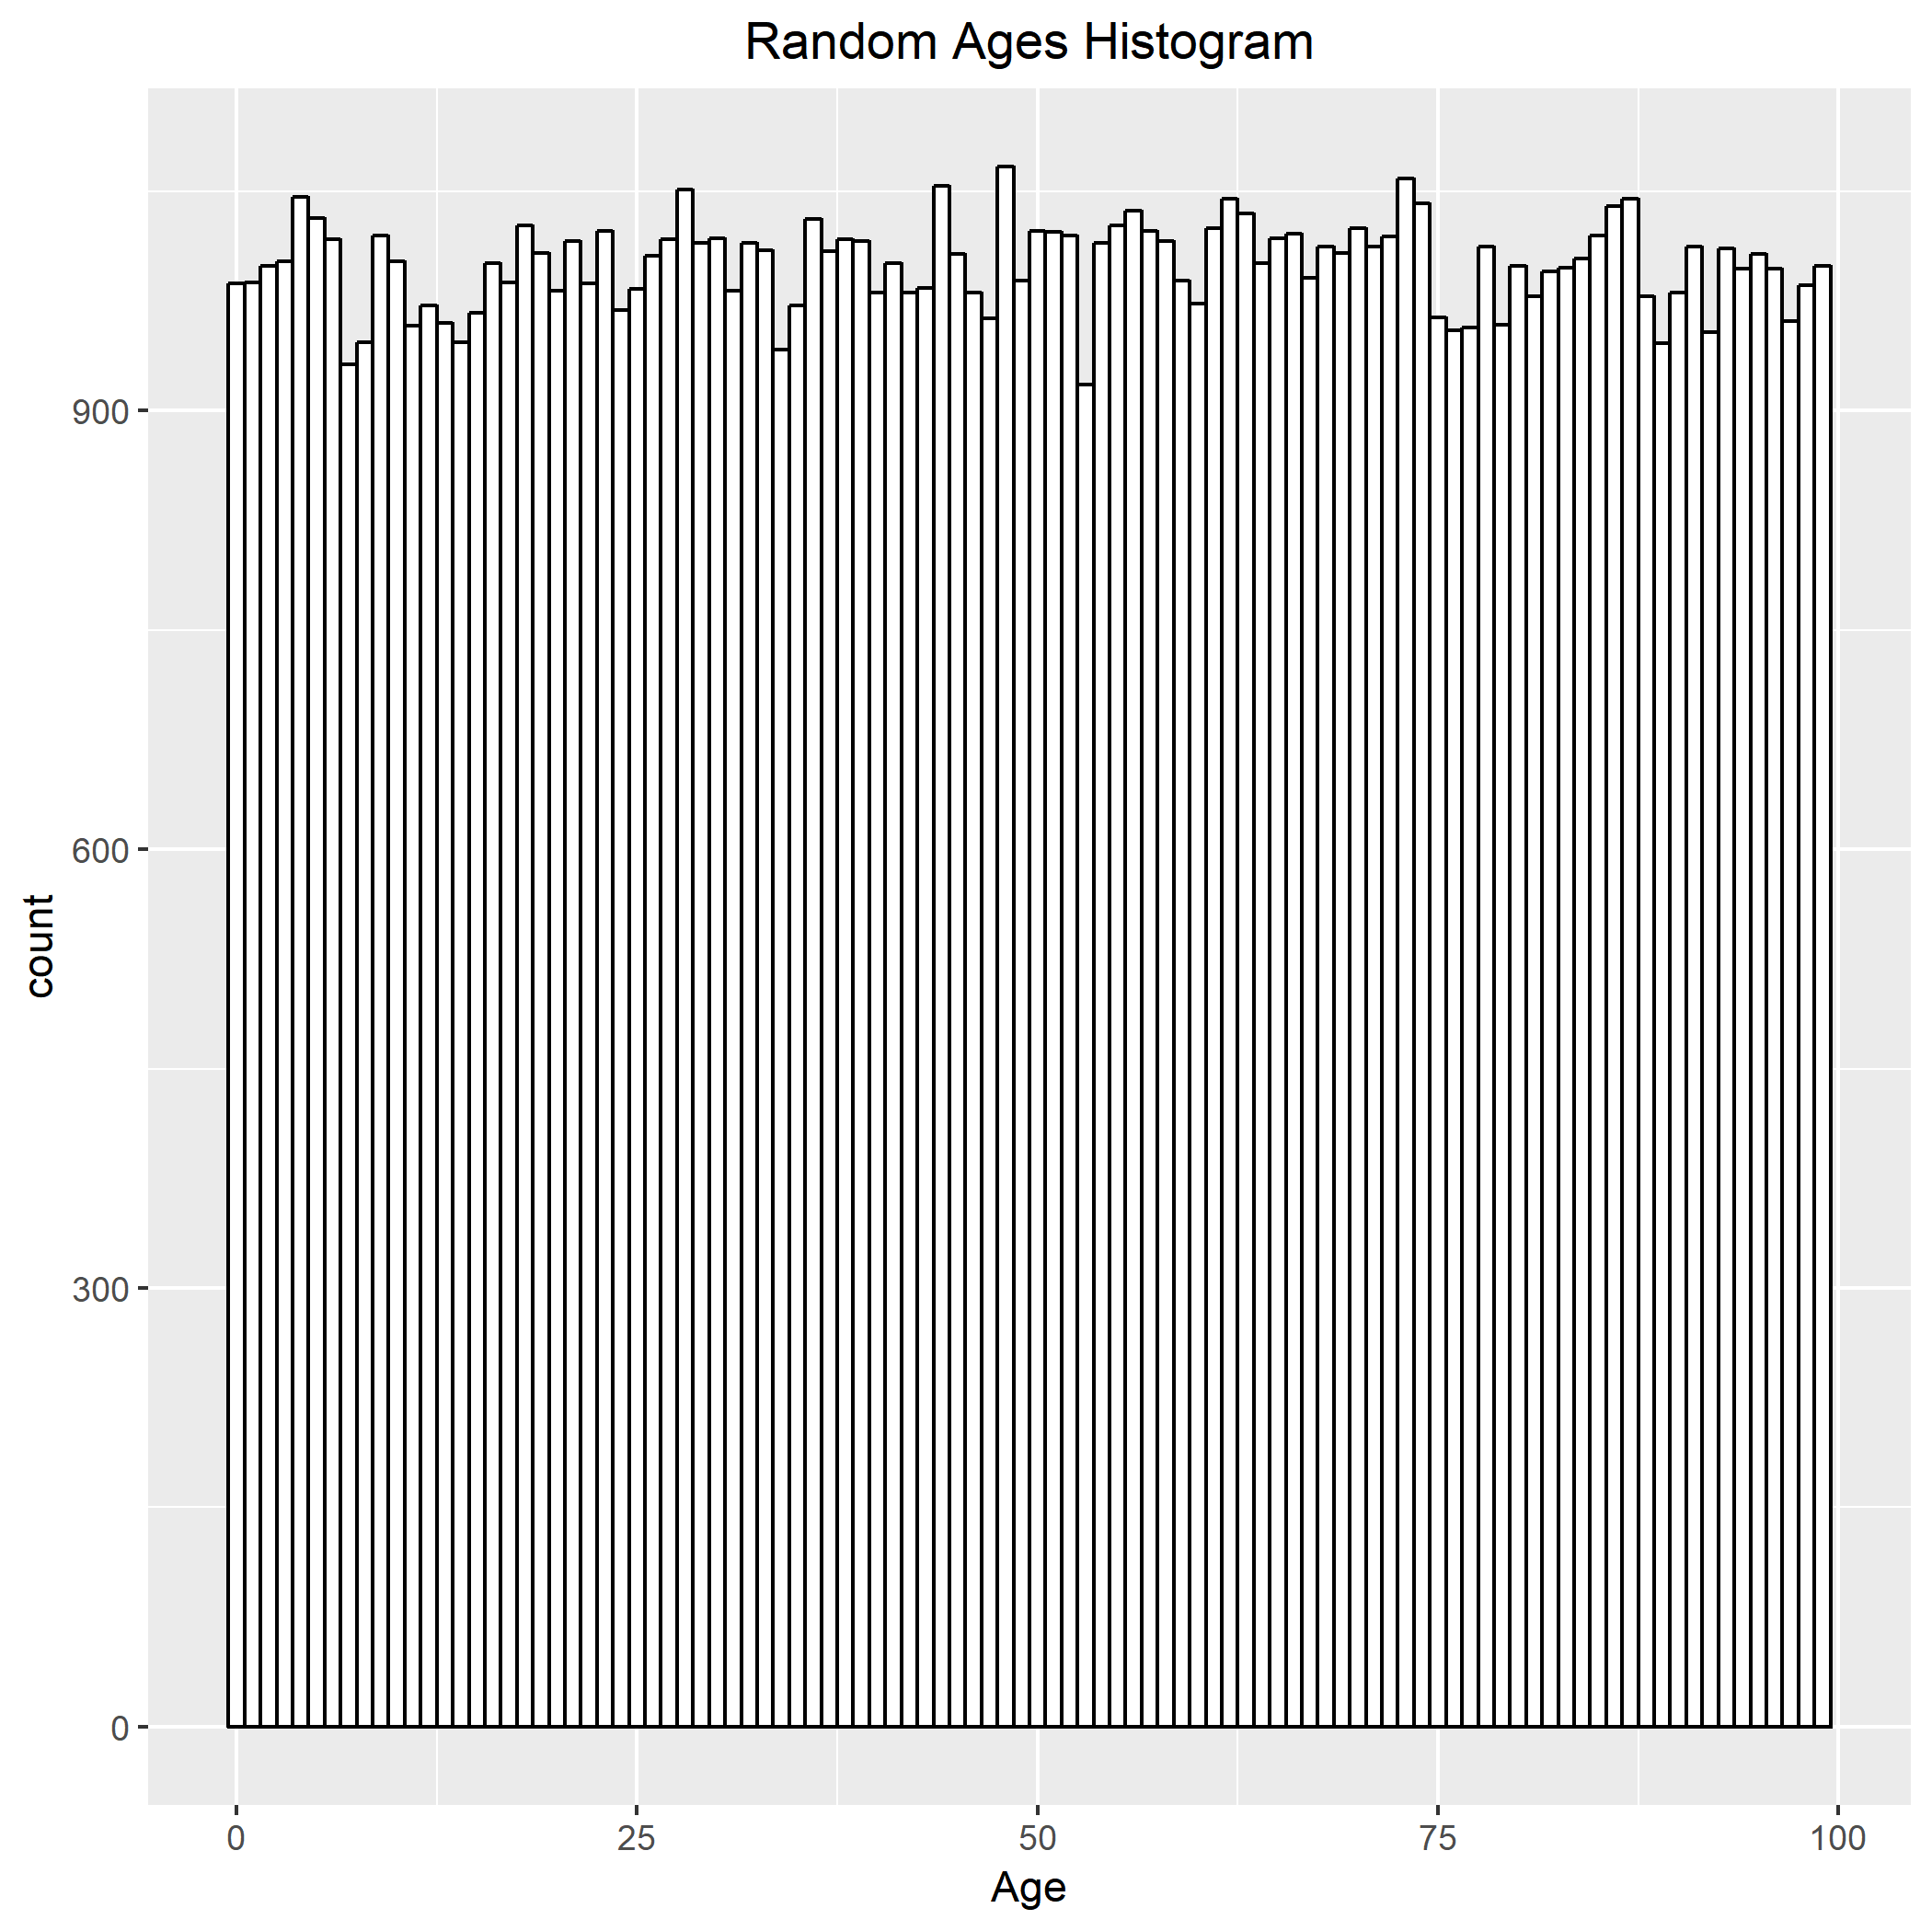
\includegraphics[width=0.5\linewidth, height=5cm]{S2.png}
	\caption{Random Ages Histogram }
	
\end{figure}




\begin{lstlisting}[caption={Random Benefit Histogram}]
x11()
myGraph <- ggplot(bDataFrame, aes(Benefit))
myGraph <- myGraph + geom_histogram(colour="black", fill="white") + labs(title = "Random Benefit Histogram")
print(myGraph)
ggsave(filename = "images/Random Benefit Histogram.png", plot = myGraph)
\end{lstlisting}

\begin{figure}[h]
	\centering
	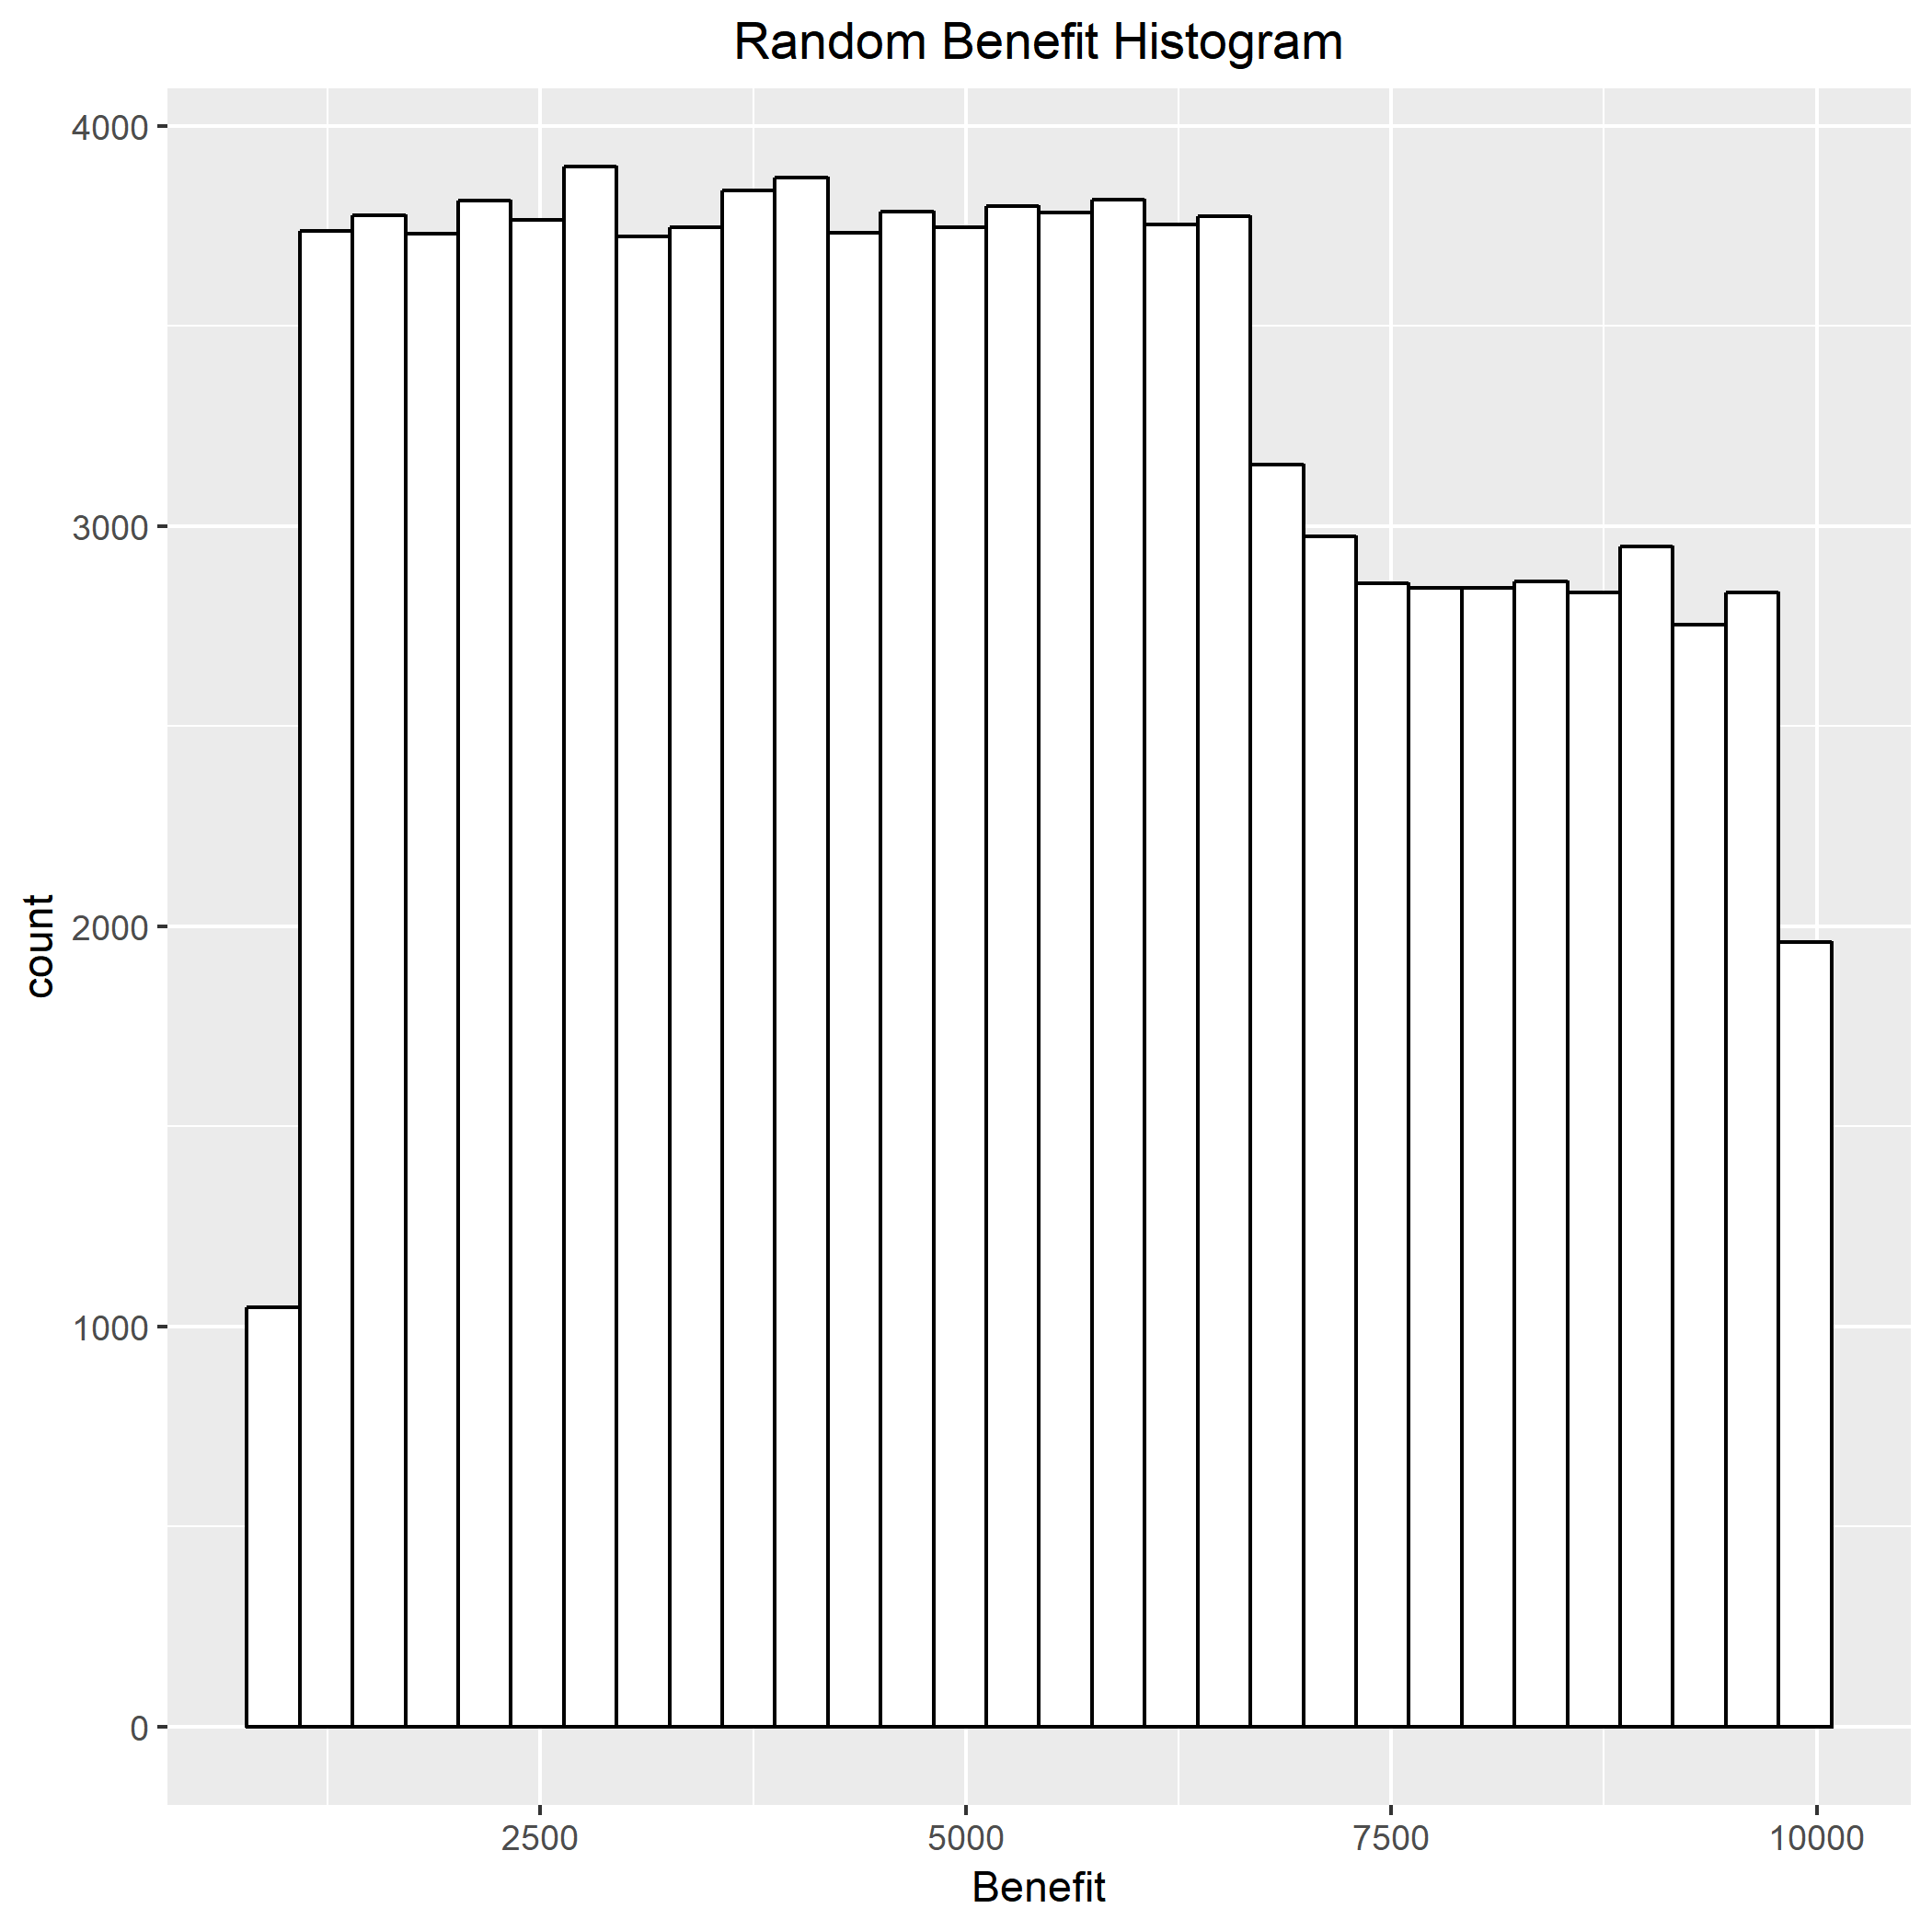
\includegraphics[width=0.5\linewidth, height=5cm]{S3.png}
	\caption{Random Benefit Histogram }
	
\end{figure}
\pagebreak
\begin{lstlisting}[caption={ Random Net Single Premium Histogram},captionpos=b]
x11()
myGraph <- ggplot(bDataFrame, aes(NetSinglePremium))
myGraph <- myGraph + geom_histogram(colour="black", fill="white") + labs(title = "Random Net Single Premium Histogram")
print(myGraph)
ggsave(filename = "images/Random Net Single Premium Histogram.png", plot = myGraph)
\end{lstlisting}
\begin{figure}[h]
	\centering
	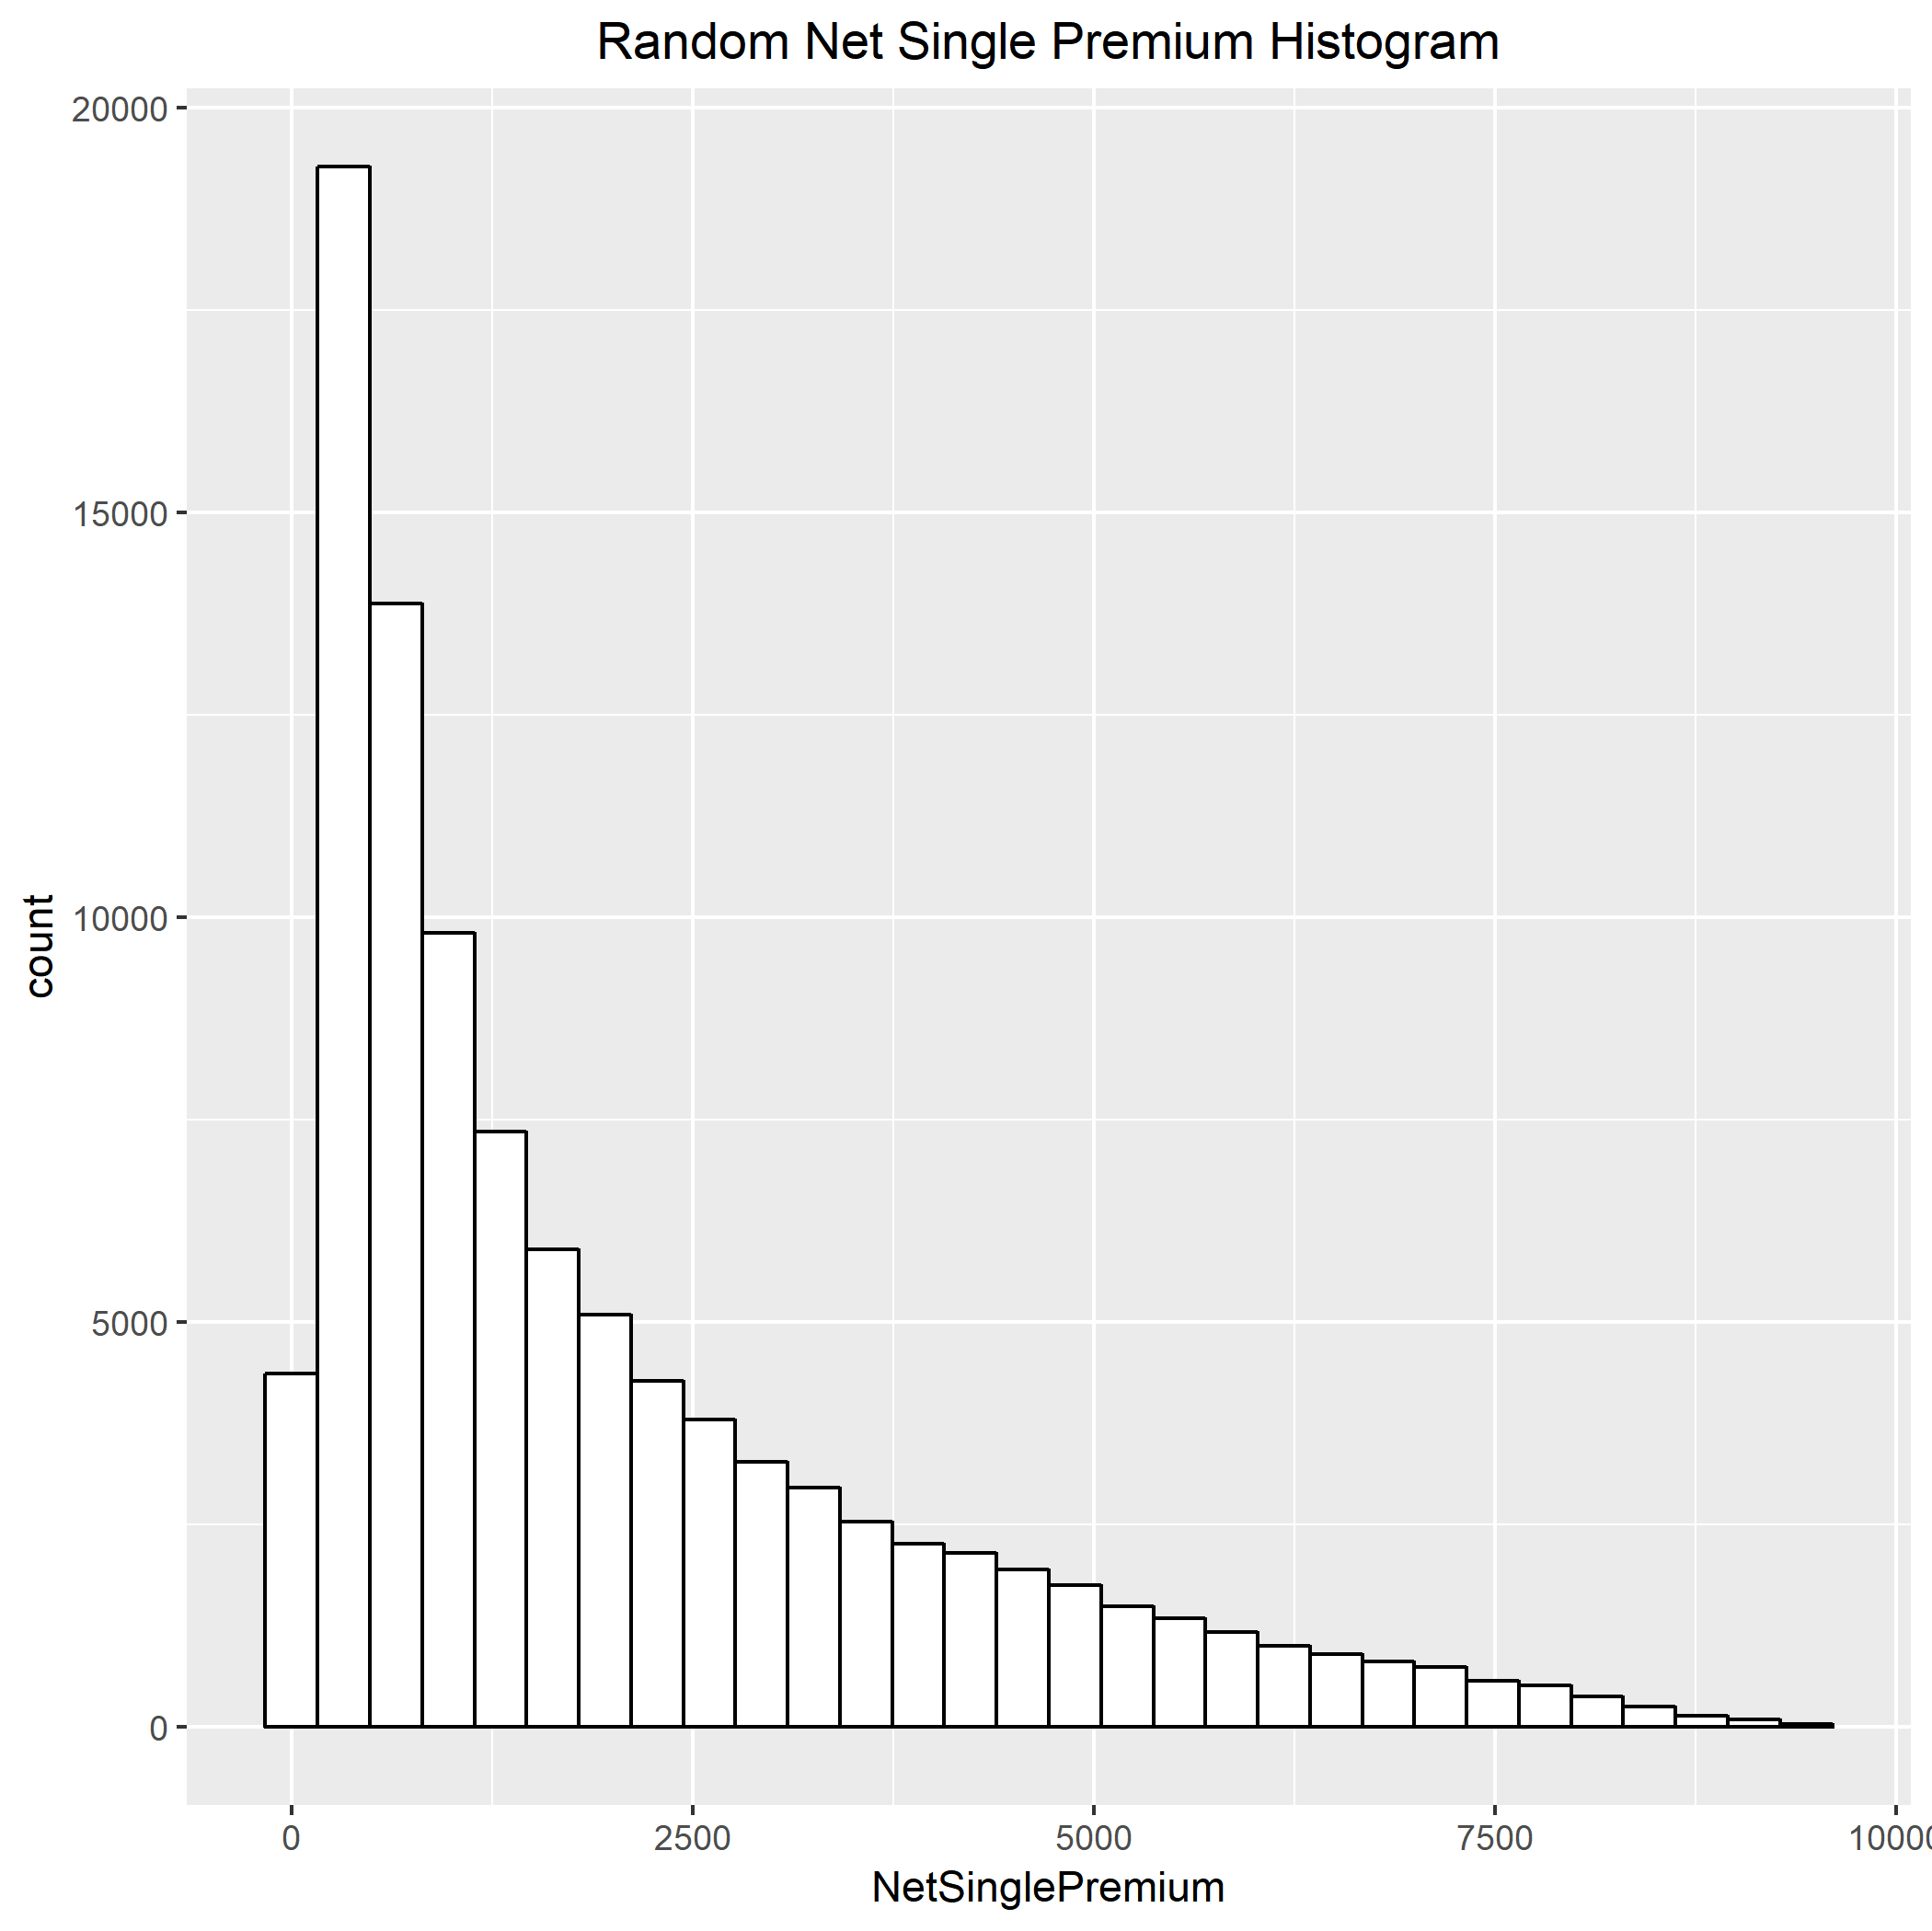
\includegraphics[width=0.5\linewidth, height=5cm]{S4.png}
	\caption{Random Net Single Premium Histogram }
	
\end{figure}

\begin{lstlisting}[caption={Random Death Ages Histogram},captionpos=b]
x11()
myGraph <- ggplot(bDataFrame, aes(Die))
myGraph <- myGraph + geom_histogram(binwidth=1, colour="black", fill="white") + labs(title = "Random Dead Ages Histogram")
print(myGraph)
ggsave(filename = "images/Random Dead Ages Histogram.png", plot = myGraph)
\end{lstlisting}
\begin{figure}[h]
	\centering
	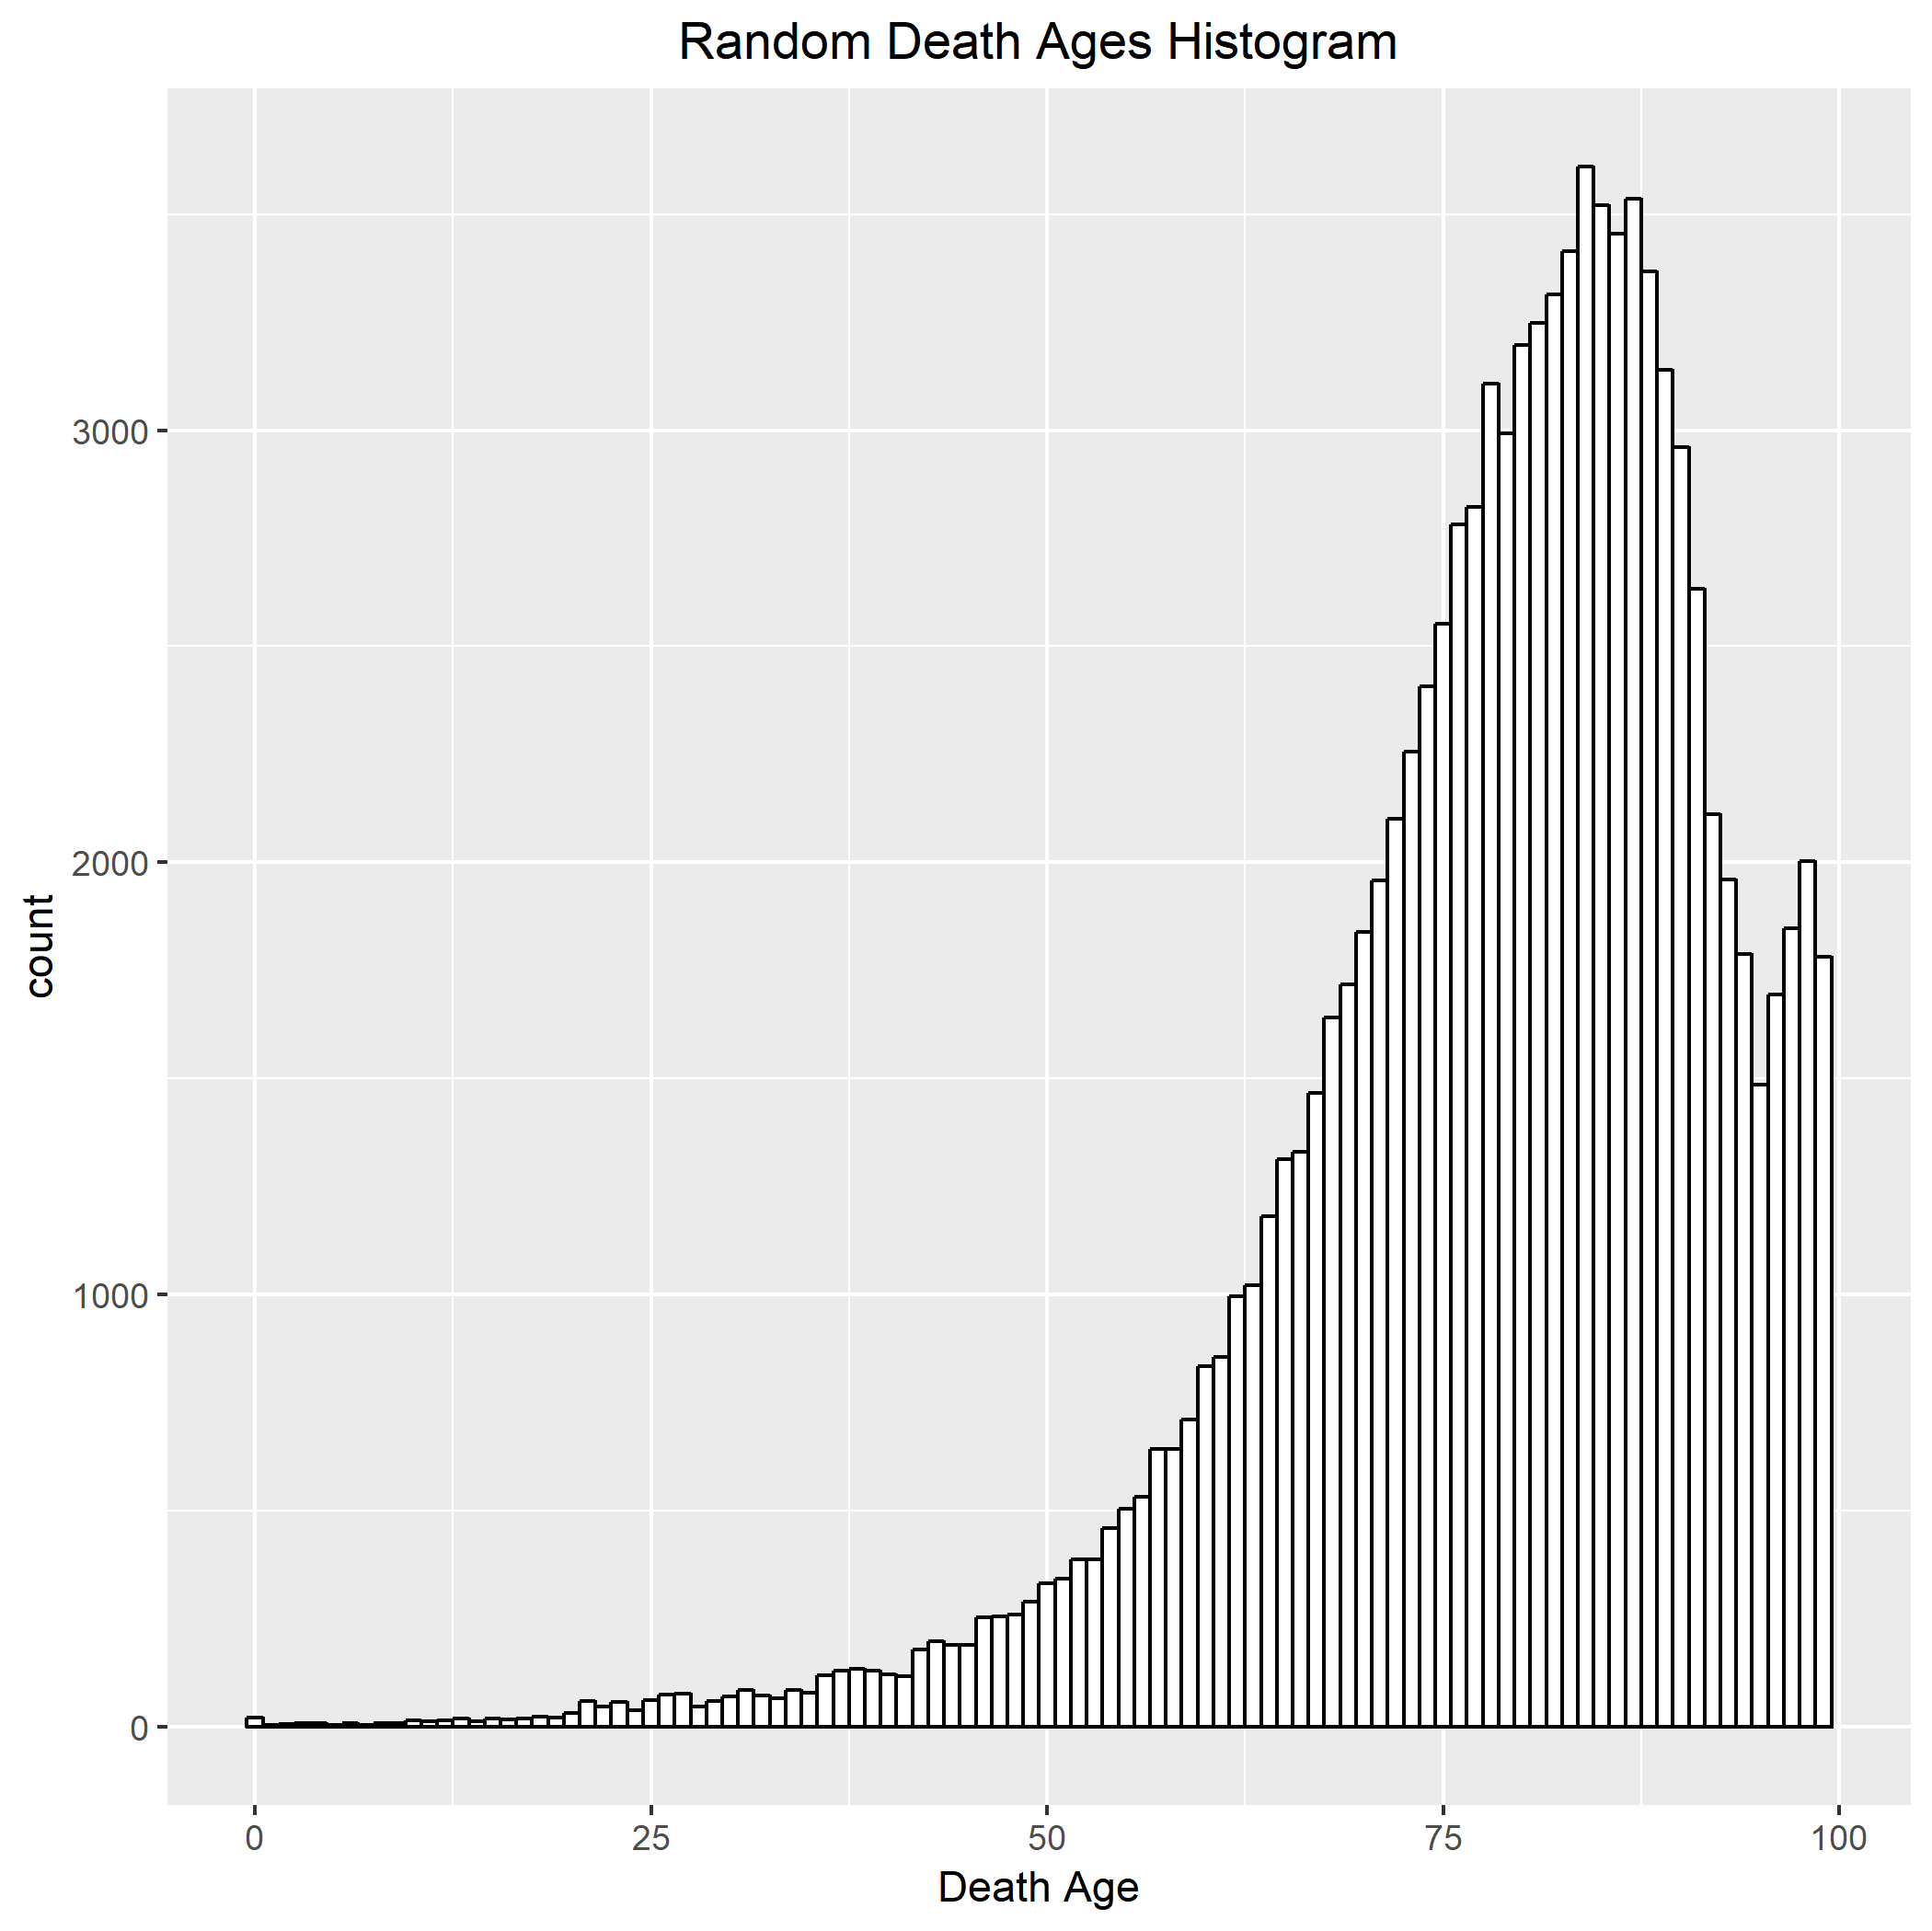
\includegraphics[width=0.5\linewidth, height=5cm]{S5.png}
	\caption{Random Death Ages Histogram}
	
\end{figure}
\pagebreak
\begin{lstlisting}[caption={Random Survived Years Histogram},captionpos=b]
x11()
myGraph <- ggplot(bDataFrame, aes(SurviveYears))
myGraph <- myGraph + geom_histogram(binwidth=1, colour="black", fill="white") + labs(title = "Random Survive Years Histogram")
print(myGraph)
ggsave(filename = "images/Random Survive Years Histogram.png", plot = myGraph)
\end{lstlisting}
\begin{figure}[h]
	\centering
	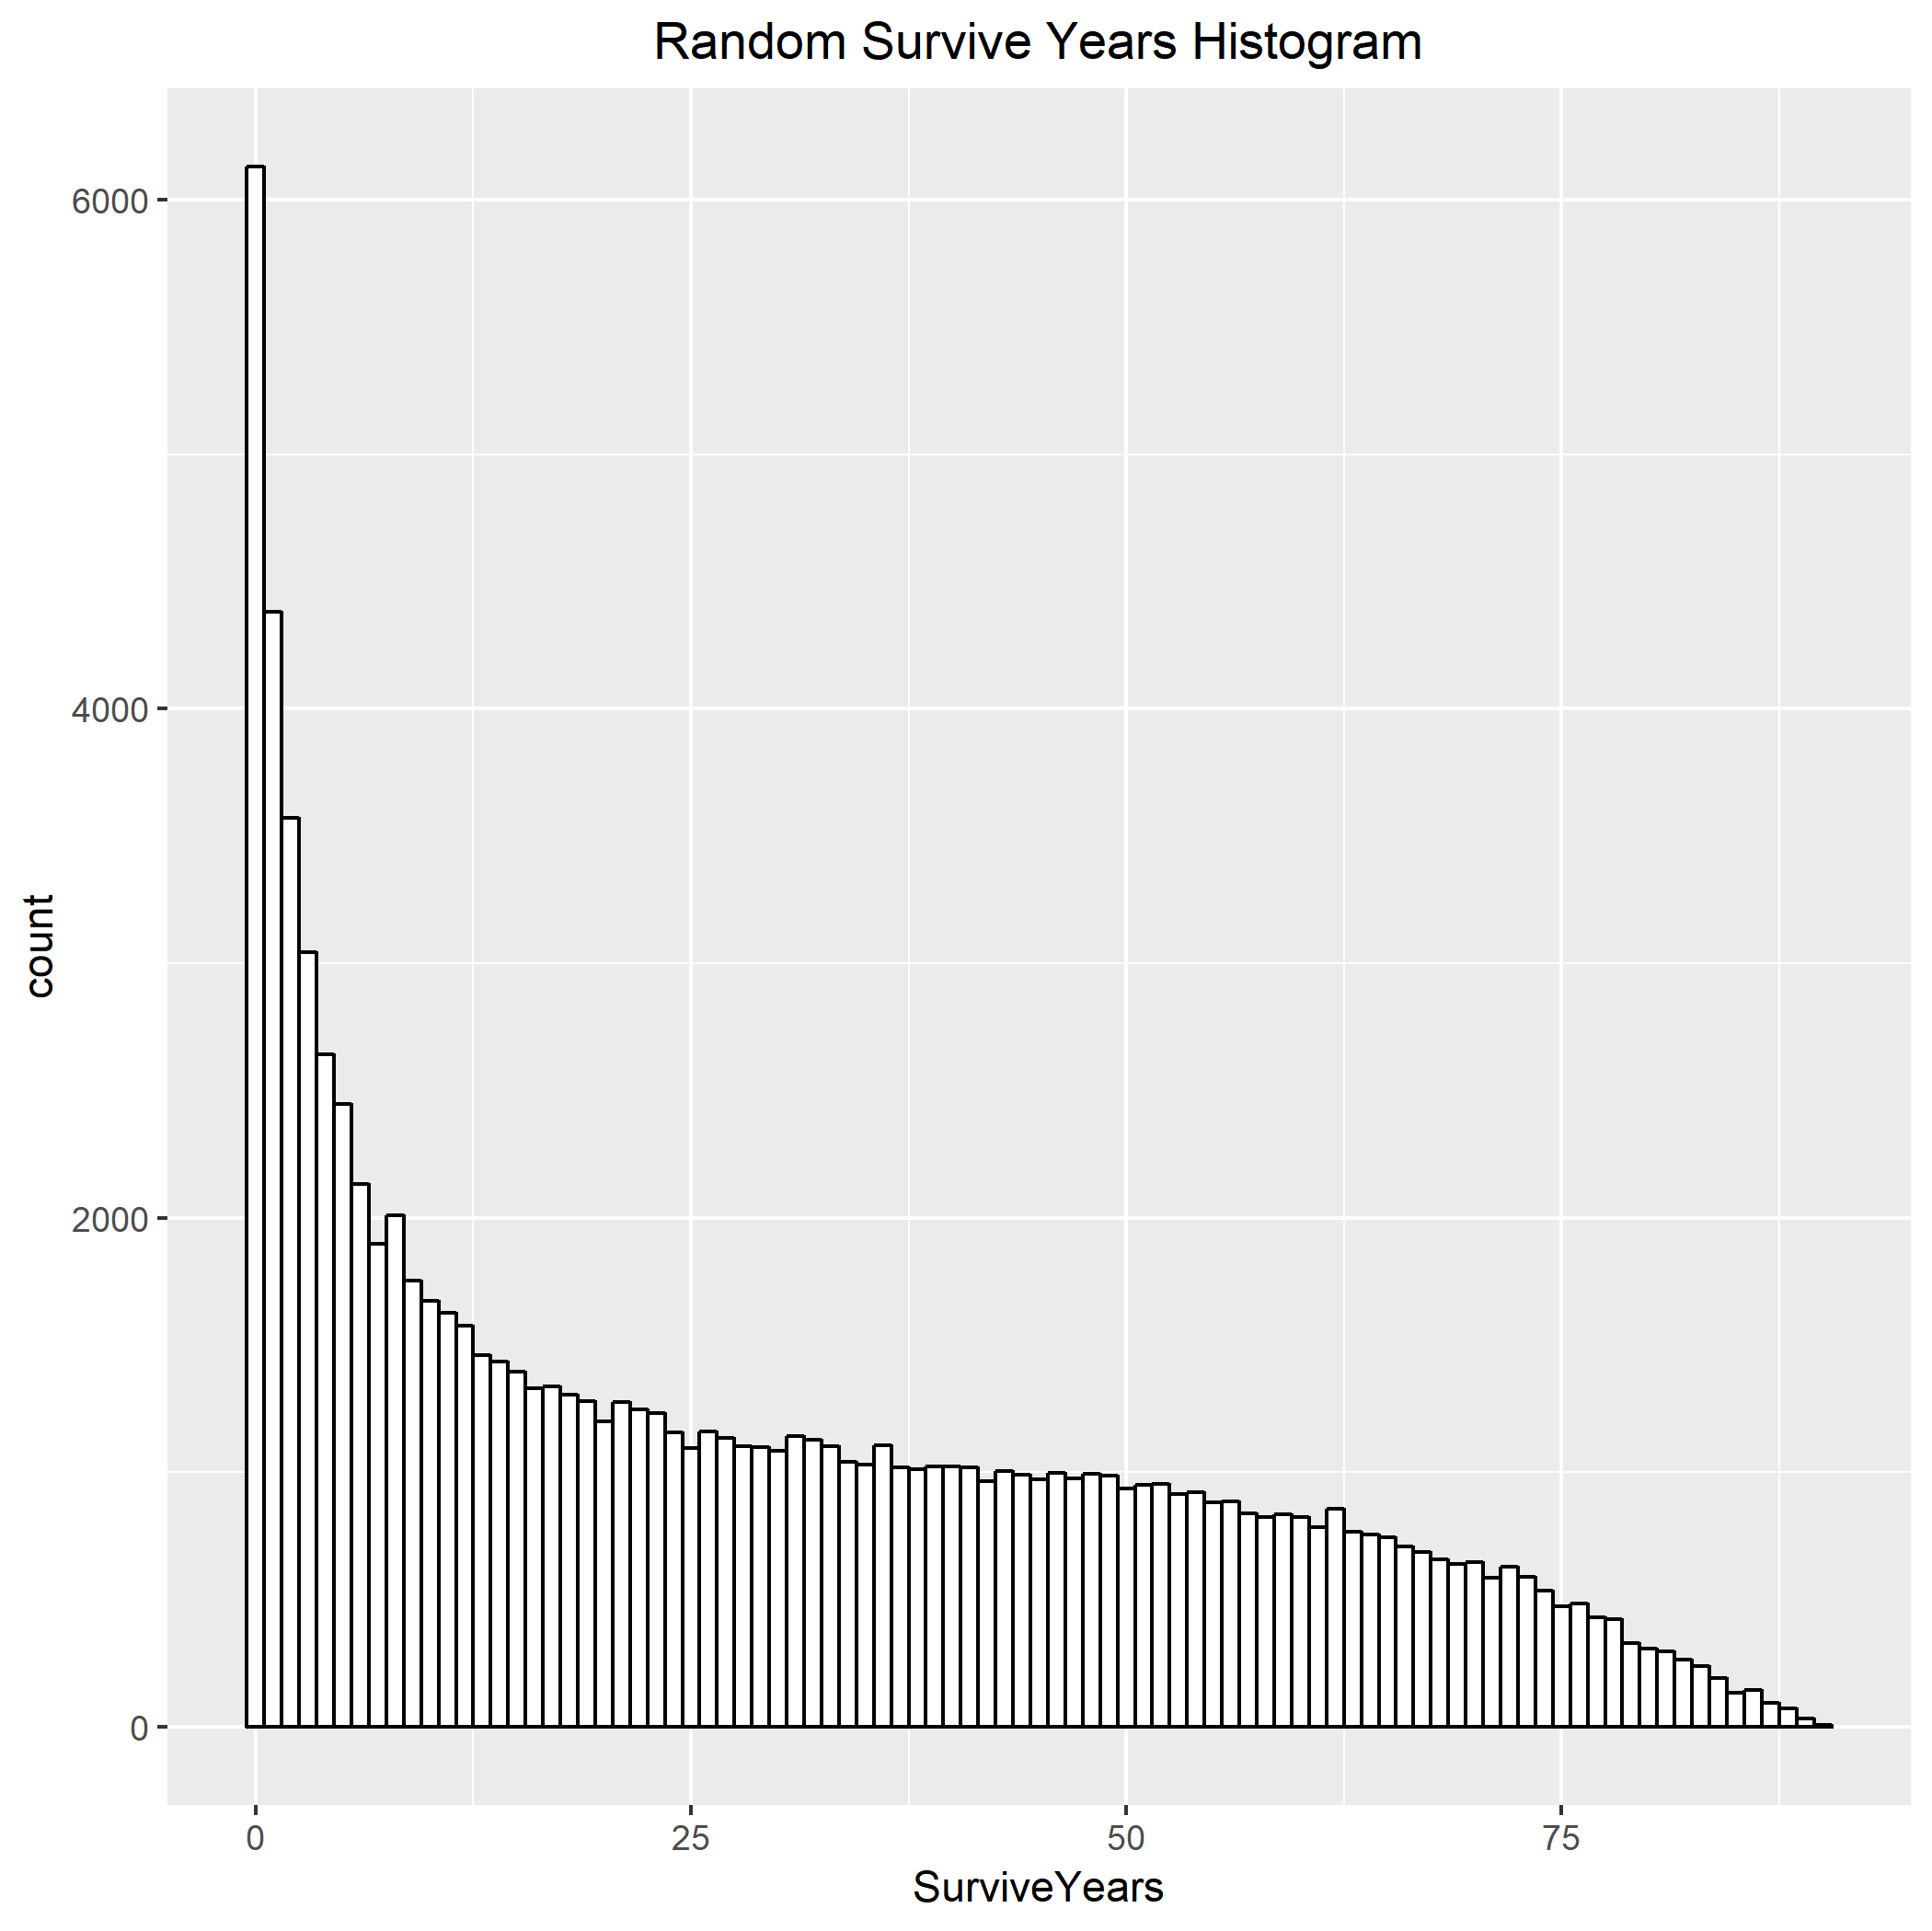
\includegraphics[width=0.5\linewidth, height=5cm]{S6.png}
	\caption{Random Survived Years Histogram}

\end{figure}
\pagebreak
\begin{lstlisting}[caption={Company Profit Graph},captionpos=b]
#------------------- print profit graph ------------------
meltProfitTable <- melt(profitTable, id="surviveYears")
x11()
myGraph <- ggplot(meltProfitTable, aes(x = surviveYears, y = value, colour = variable))
myGraph <- myGraph + geom_point() + labs(title="Company Profit Graph", y = "Money [$US]") + geom_line(linetype = "dashed") +
scale_color_manual(labels = c("Profit", "Interest", "Payment"), values = c("Green","blue", "red")) 
print(myGraph)

ggsave(filename = "images/Company Profit Graph.png", plot = myGraph)

endTime <- Sys.time() # calulating the ending time
totalTime <- endTime - startTime #calulating the total time
print(totalTime) # printing the total time
\end{lstlisting}
In Listing 15, Line 2 uses one of the reshapes's library functions. Melt function which allows you to plot more that one thing on the same window. As mentioned earlier x11() function opens a new graph window before creating a new graph to avoid overwriting of previous plotted graphs. Line 4 sets the axis of the plot. Line 5 sets the title and the plot will be plotted as lines and sets the legend of the plot. Line 7 displays the graph on the screen. Line 9 saves the graph on images directory which should be created on the same working directory. Line 11 stores the time when the code is ended its execution. Line 12 calculates the total time . Line 13 prints the total time. Figure 7 shows the output of line 7.
\clearpage
\begin{figure}[h]
	\centering
	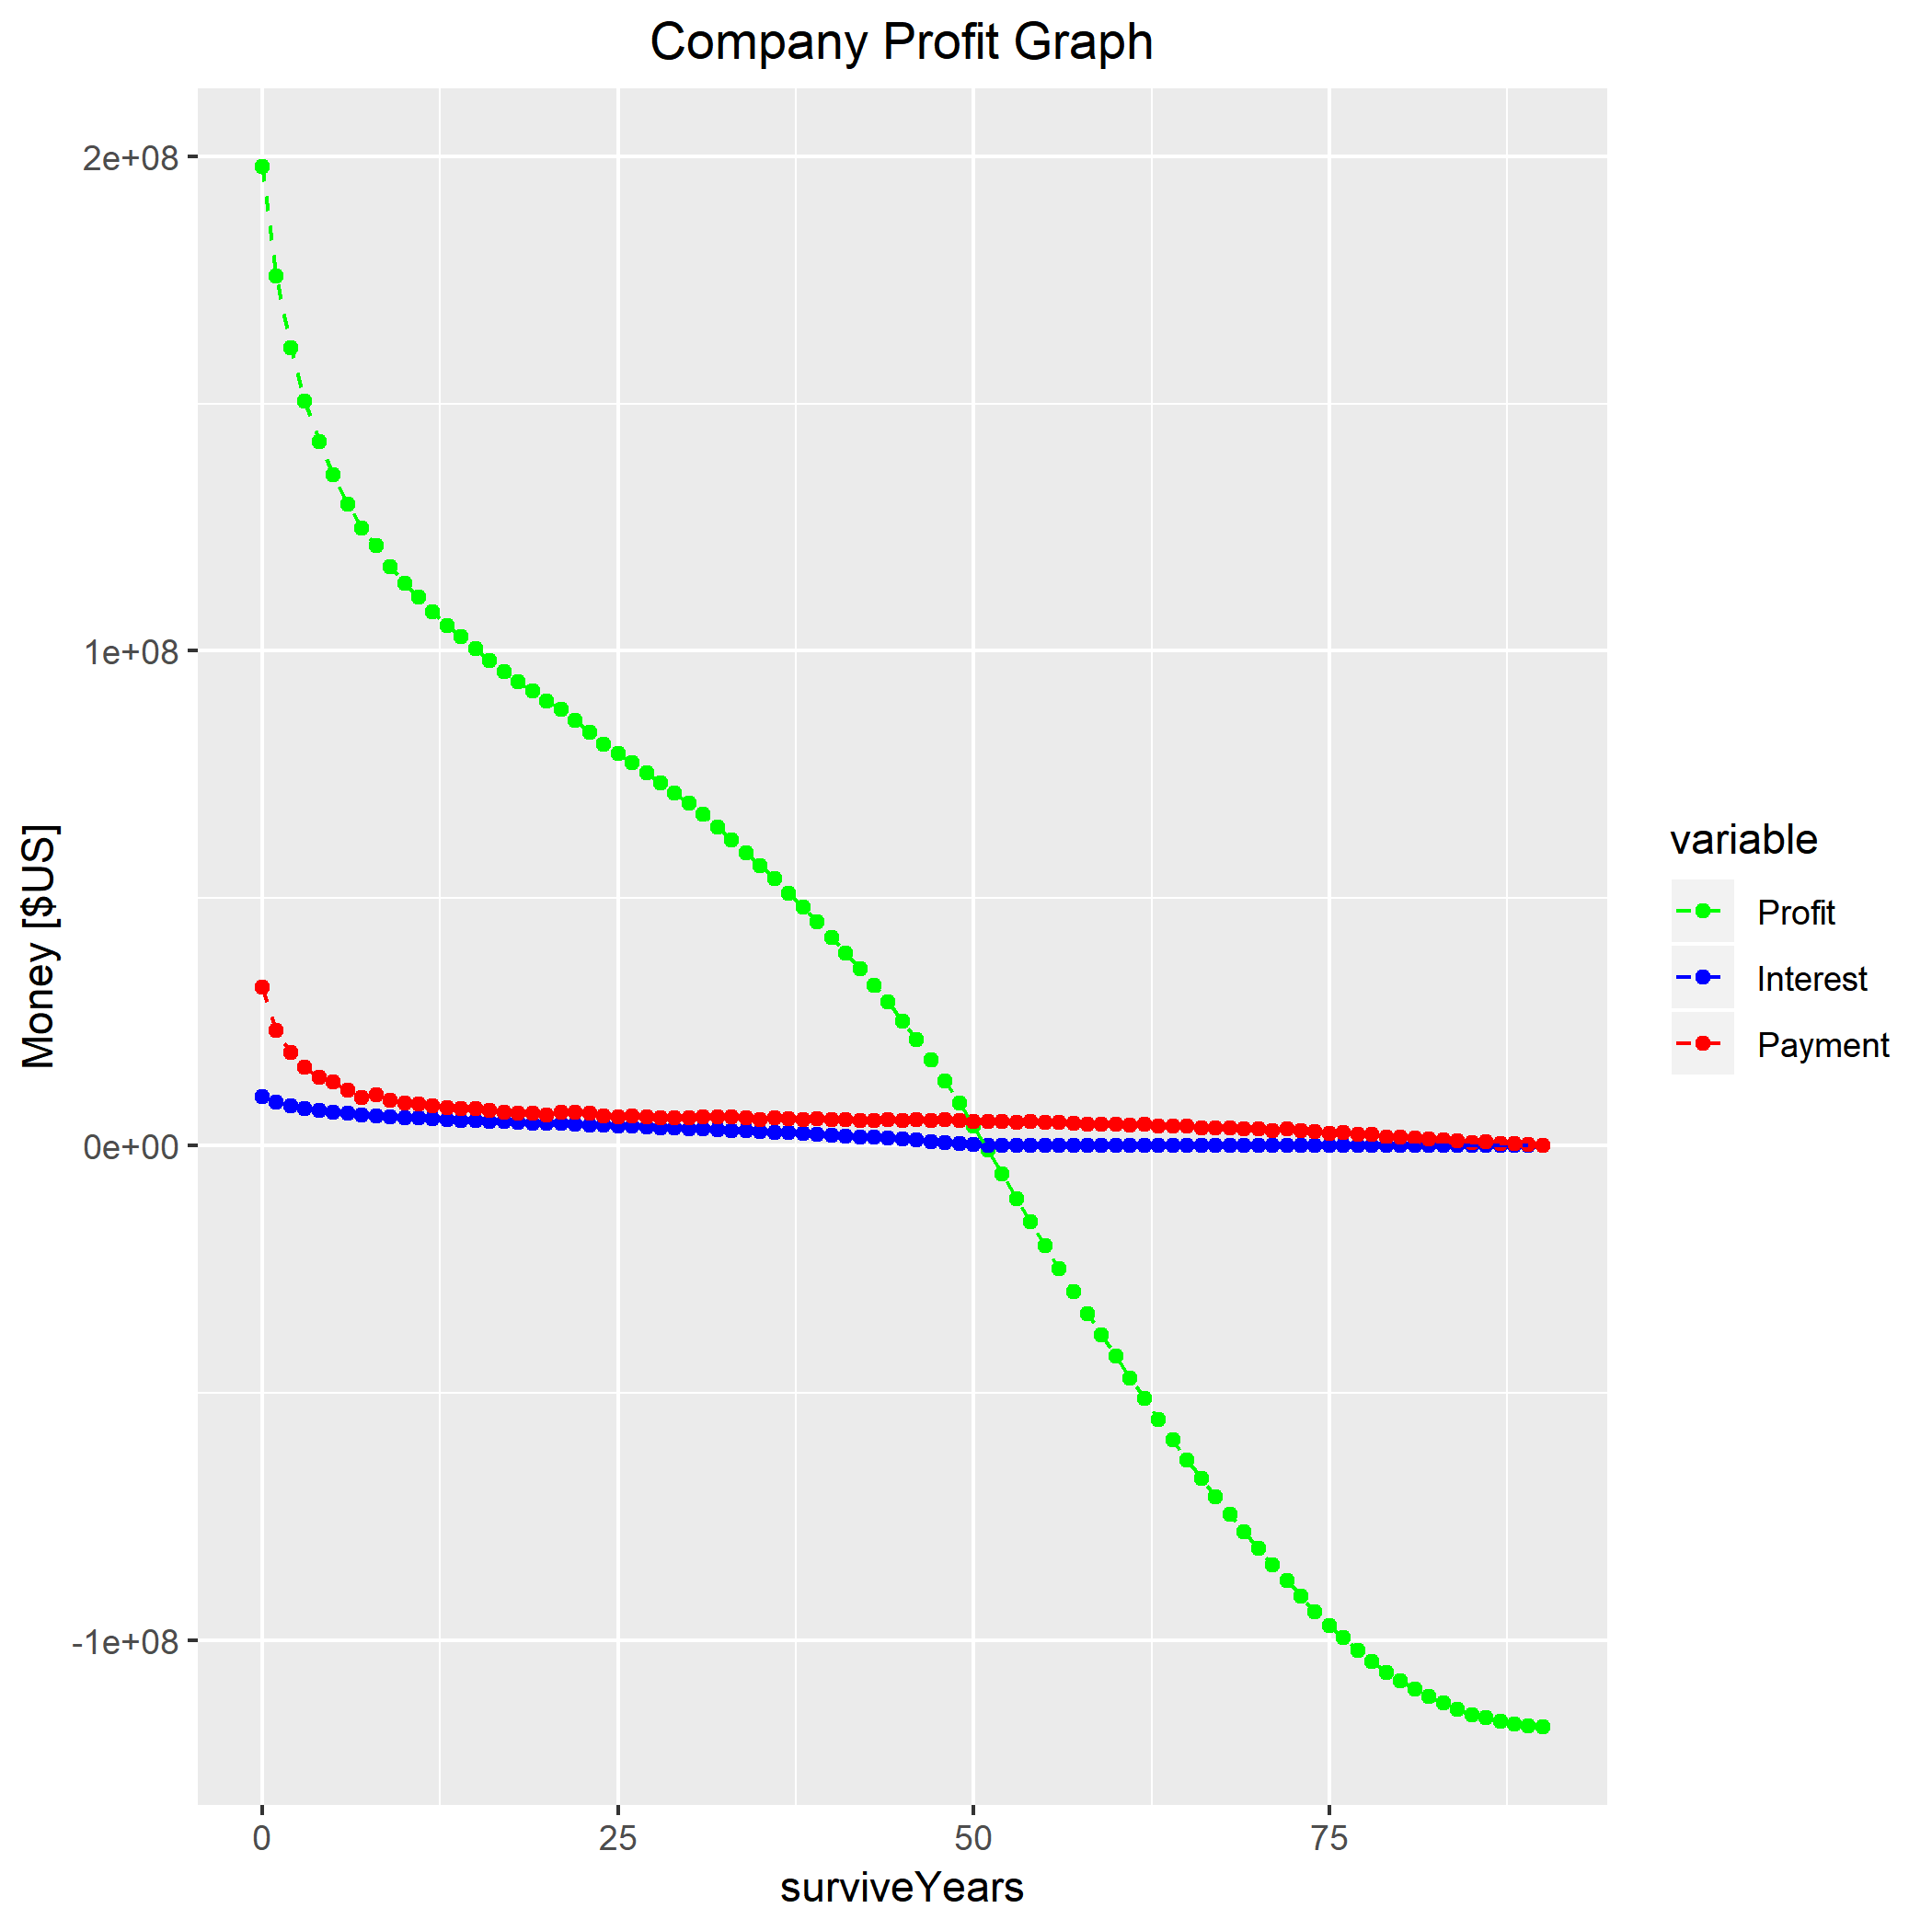
\includegraphics[width=0.7\linewidth, height=7cm]{S7.png}
	\caption{Company Profit Graph}

\end{figure}
\begin{lstlisting}[caption={Calculating The Fund Value},captionpos=b]
# Now, claulating the Fund value:
# F(t)= Premium (t)+ accumlatedMonthlyinterest(t)- benefit(t)
for (i in 1:(tTimes-1)) {
fundValues[i+1] <- fundValues[i] + interestMonthBased[i] - benefitPay[i]
if(fundValues[i+1] > 0){ #only calculate Interest when fund > 0
interestMonthBased[i+1] <- fundValues[i+1] * (1+investmentInterest/12)^12 - fundValues[i+1] 
}
else {
interestMonthBased[i+1] <- 0
}
accInterMonthBased[i+1] <- accInterMonthBased[i] +  interestMonthBased[i+1]
accBenPay[i+1] <- accBenPay[i] +  benefitPay[i+1]
}
fundValueTable<-data.frame(year,fundValues, interestMonthBased, benefitPay, accInterMonthBased, accBenPay)
\end{lstlisting}
\pagebreak
The code in listing 16 calculates the fund value introduced in equation 3. Lines 3-12 loop through the number of survived years and calculate the fund value according to equation 3.  The monthly interest is calculated as well. The code stores the fund values and monthly interests in \textit{fundValues} and \textit{interestMonthBased} respectively. Line 14 creates a data frame called \textit{fundValuesTable} that contains the year, fund values, monthly interest, benefit payment, accumulated monthly interest and accumulated benefit payment.
\begin{equation}
F(t)= Premium (t)+ accumlatedMonthlyinterest(t)- benefit(t)
\end{equation}
\begin{lstlisting}[caption={Calculating The Fund Value Based on Different Interests},captionpos=b]
interestSeq <- seq(0.05, 0.055, 0.0005)
yearSeq <- fundValueTable$year
matrixFund <- matrix(, nrow = length(yearSeq), ncol = length(interestSeq)) # empty matrix
column <- 1

for (i in interestSeq){
matrixFund[,column] <- CalculateFundValue(i)$fundValues
column <- column + 1
}
\end{lstlisting}
The code in listing 17 is similar to the code in listing 16 except that listing 17 calculates the fund value based on a variety of interest. The first loop calculates the fund value based in 0.05\% interest. The second loop calculates the fund value based in 0.055\% interest. The third loop calculates the fund value based in 0.0005\% interest. The code stores the results in a matrix for a 3D surface plotting. Below is a gif message that visualizes the outcome.

\animategraphics[controls,autoplay,loop,width=1\linewidth]{12}{Fund3DG/ez-}{0}{309}

\begin{lstlisting}[caption={Calculating The Reserve Value },captionpos=b]
nrowbDataFrame <- nrow(bDataFrame)
reserveTable <- data.frame(matrix(ncol = 3, nrow = nYears))
colnames(reserveTable) <- c("SurviveYears", "Reserve", "NumberPolicies")
for (reserveYear in 1:nYears){
counter<-0
reserveAmount <- 0
for (i in 1:nrowbDataFrame){
if (bDataFrame$SurviveYears[i] >= reserveYear)
{counter <- counter + 1 
#t_V = 1 - a_(x+t)/a_x
x <- bDataFrame$Age[i]
A_x_t <- lifeTable$A_x[(x+1+reserveYear)] # faster
t_V <- A_x_t
reserveAmount <- reserveAmount + bDataFrame$Benefit[i]*t_V
}}
reserveTable$SurviveYears[reserveYear] <- reserveYear-1
reserveTable$NumberPolicies[reserveYear] <- counter
reserveTable$Reserve[reserveYear] <- reserveAmount
}
\end{lstlisting}
Listing 18 computes the reserve value based on equation 4.
\begin{equation}
_{s}V=A_{x+s}
     = EPV [Benefit]
     =\sum_{k=1}^{\infty}V^{k+1} * _{k1}q_{x+3}
\end{equation}
\begin{equation}
Profit= Premium + Yearly Interests - Benefit Payment
\end{equation}
\begin{lstlisting}[caption={Calculating The Annual Profit and The Reserve Value },captionpos=b]
#find payment of the year 0
payment <- paymentTable[paymentTable$SurviveYears == 0, c("Benefit")] 
if(length(payment) == 0){ #sometime there is no payment for specific year, so convert numeric(0) to 0
benefitPayment[1] <- 0
}else{
benefitPayment[1] <- payment
}
#find reserve of the year 0
reserve <- reserveTable[reserveTable$SurviveYears ==0, c("Reserve")]
if(length(reserve) == 0){ #sometime there is no reserve for specific year, so convert numeric(0) to 0
reserveHold[1] <- 0
}else{
reserveHold[1] <- reserve
}
surviveYears <- vector(mode="integer", length=(nYears+1))
surviveYears[1] <- 0
for (i in 1:nYears) {
surviveYears[i+1] <- i
money[i+1] <- money[i] + earnInterest[i] - benefitPayment[i] 
if(money[i+1] > 0){ #only calculate earnInterest when money > 0
earnInterest[i+1] <- money[i+1]*investmentInterest
}
else {
earnInterest[i+1] <- 0
}
#find payment of next year
payment <- paymentTable[paymentTable$SurviveYears == i, c("Benefit")] 
if(length(payment) == 0){ #sometime there is no payment for specific year, so convert numeric(0) to 0
benefitPayment[i+1] <- 0
}
else{
benefitPayment[i+1] <- payment
}
#find reserve of next year
reserve <- reserveTable[reserveTable$SurviveYears == i, c("Reserve")]
if(length(reserve) == 0){ #sometime there is no reserve for specific year, so convert numeric(0) to 0
reserveHold[i+1] <- 0
}else{
reserveHold[i+1] <- reserve
}} 
profitTable <- data.frame(surviveYears, money, earnInterest, benefitPayment, reserveHold)
#calculate  profit
profitTable$profit <- profitTable$money + profitTable$earnInterest - profitTable$benefitPayment - profitTable$reserveHold
\end{lstlisting}


\animategraphics[controls,autoplay,loop,width=1\linewidth]{12}{Fund3DG/ezo-}{0}{296}

Listing 19 calculates the yearly profit along with the annual reserve based on equation 4 and equation5. The gif image above visualizes the outcome. Figure 8 shows profit graphs of the project. Since we generate the benefit randomly, the profit graph will have different shape each time we run the code.
\begin{figure}[h]
	\begin{tabular}{cc}
		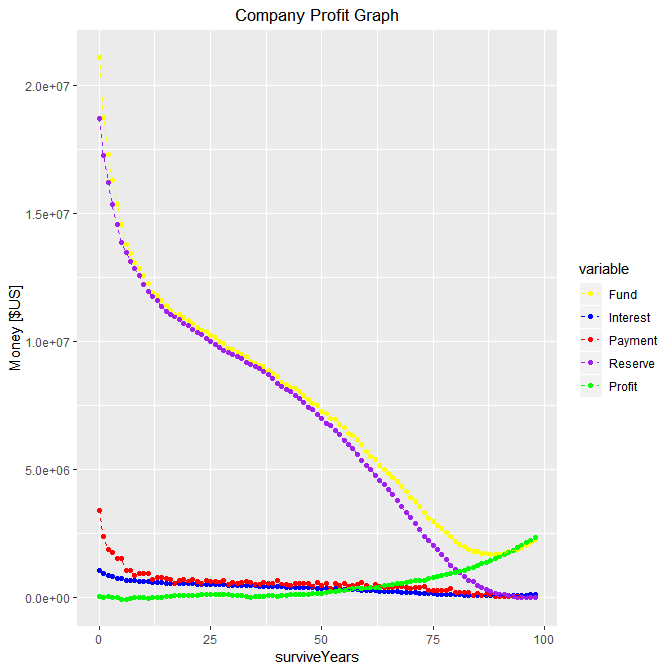
\includegraphics[width=65mm]{report_profit.PNG} &   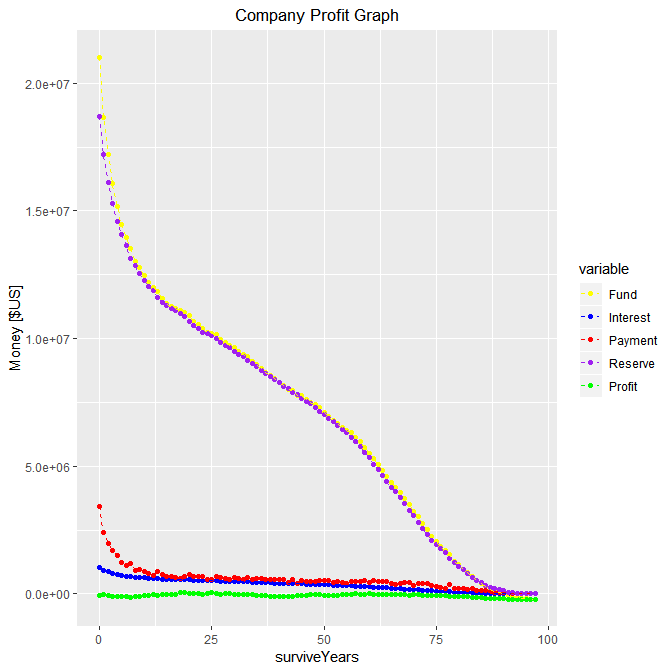
\includegraphics[width=65mm]{profit1.PNG} \\
		(a) first & (b) second \\[6pt]
		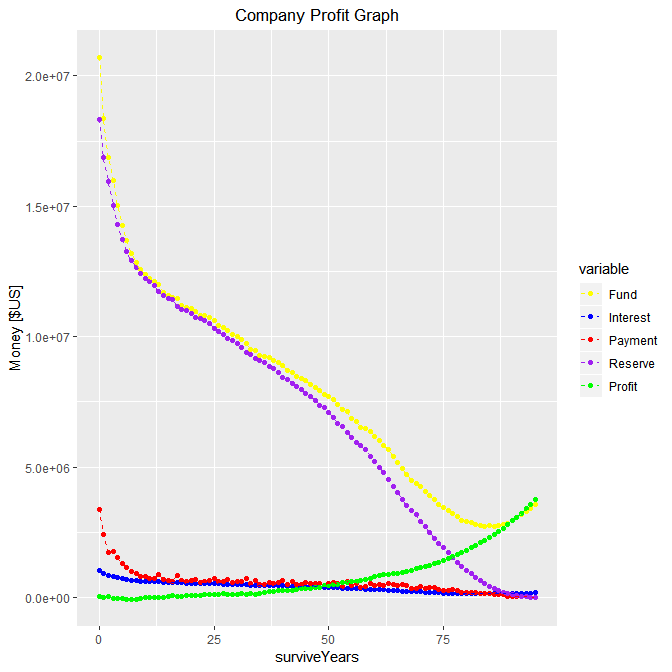
\includegraphics[width=65mm]{profit2.PNG} &   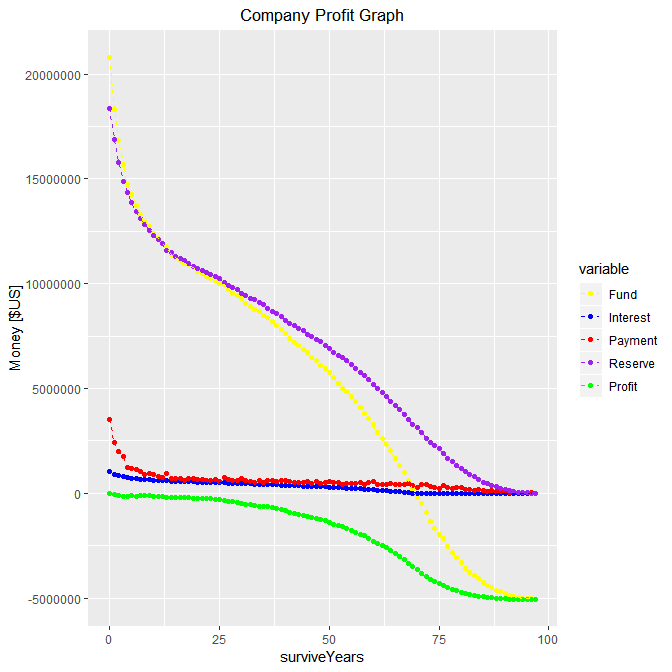
\includegraphics[width=65mm]{profit3.PNG} \\
		(c) third & (d) fourth \\[6pt]

	\end{tabular}
	\caption{Profit Graphs}
\end{figure}

\end{document}

